\documentclass[11pt]{amsart}
\usepackage[T1]{fontenc}
\usepackage{lmodern}
\usepackage[margin=1.15in]{geometry}
\usepackage{amsmath,amssymb,amsthm,mathtools}
\usepackage[authoryear,round]{natbib}
\usepackage{enumitem}
\usepackage{booktabs}
\usepackage{tikz}
\usetikzlibrary{positioning}
\usepackage[colorlinks=true,linkcolor=blue,citecolor=blue,urlcolor=blue]{hyperref}
\setlength{\emergencystretch}{2em}

% ---------------------------------------------------------------- theorem environments
\newtheorem{theorem}{Theorem}[section]
\newtheorem{proposition}[theorem]{Proposition}
\newtheorem{lemma}[theorem]{Lemma}
\newtheorem{corollary}[theorem]{Corollary}
\newtheorem{mainthm}{Theorem}
\renewcommand{\themainthm}{\Alph{mainthm}}
\newtheorem{maincor}[mainthm]{Corollary}
\newtheorem{mainprop}[mainthm]{Proposition}
\newtheorem*{conjecture*}{Christol's conjecture}
\theoremstyle{definition}
\newtheorem{definition}[theorem]{Definition}
\newtheorem{example}[theorem]{Example}
\theoremstyle{remark}
\newtheorem{remark}[theorem]{Remark}
\numberwithin{equation}{section}

% ---------------------------------------------------------------- notation
\newcommand{\Q}{\mathbb{Q}}
\newcommand{\Z}{\mathbb{Z}}
\newcommand{\C}{\mathbb{C}}
\newcommand{\R}{\mathbb{R}}
\newcommand{\Qb}{\overline{\mathbb{Q}}}
\newcommand{\PP}{\mathbb{P}}
\newcommand{\A}{\mathbb{A}}
\newcommand{\e}{\mathbf{e}}
\newcommand{\cS}{\mathcal{S}}
\newcommand{\cX}{\mathcal{X}}
\newcommand{\cO}{\mathcal{O}}
\newcommand{\cD}{\mathcal{D}}
\newcommand{\cB}{\mathcal{B}}
\newcommand{\cE}{\mathcal{E}}
\newcommand{\cA}{\mathcal{A}}
\newcommand{\cT}{\mathcal{T}}
\newcommand{\tp}{\mathrm{top}}
\newcommand{\bt}{\mathrm{bot}}
\newcommand{\alg}[2]{#1\langle #2\rangle}
\newcommand{\ak}[1]{a^{(k)}_{#1}}
\newcommand{\bk}{b^{(k)}}
\DeclareMathOperator{\Diag}{Diag}
\DeclareMathOperator{\Tr}{Tr}
\DeclareMathOperator{\Hom}{Hom}
\DeclareMathOperator{\End}{End}
\DeclareMathOperator{\rank}{rank}
\DeclareMathOperator{\Spec}{Spec}
\DeclareMathOperator{\im}{Im}
\newcommand{\Fab}{F_{a,b}}
\newcommand{\Sab}{\cS_{a,b}}

\begin{document}

\title[Globally bounded ${}_3F_2$ series are diagonals]{Globally bounded ${}_3F_2$ series with one integral lower parameter are diagonals of rational functions}

\author{David Jordan}
\address{Maynooth University Social Sciences Institute (MUSSI), Maynooth University, Maynooth, County Kildare, Ireland}
\email{David.Jordan@mu.ie}

\subjclass[2020]{Primary 33C20, 14D07; Secondary 13F25, 14K10, 32G20, 05A15}
\keywords{Christol's conjecture, diagonals of rational functions, globally bounded power series, hypergeometric functions, variations of Hodge structure, abelian schemes, vanishing cycles}
\date{17 November 2026 (version 1.2)}

\begin{abstract}
Christol conjectured that every globally bounded, D-finite power series with rational coefficients is the diagonal of a rational function. We prove this for the hypergeometric series ${}_3F_2(a_1,a_2,a_3;b,1;x)$ with rational parameters such that $a_i$, $b$ and $a_i-b$ are not integers: if such a series is globally bounded, then it is the diagonal of an algebraic power series in two variables, and hence of a rational function in three variables, which is the least possible number. This includes Christol's example ${}_3F_2(\frac19,\frac49,\frac59;\frac13,1;x)$ from 1987. The proof is Hodge-theoretic and not constructive. Using Fedorov's formula for the Hodge numbers of hypergeometric local systems, we show that the series is globally bounded exactly when every Galois conjugate of its local system carries a complex variation of Hodge structure with two adjacent Hodge levels. The restriction of scalars of the local system then underlies a polarized integral variation of Hodge structure of weight one. By a theorem of Deligne the series is therefore a period of an abelian scheme, and hence of a family of curves, where it is an integral over vanishing cycles of a semistable degeneration. Expanding this integral at the nodes of a regular model gives the diagonal representation.
\end{abstract}

\maketitle

\section*{Plain-language summary}

\emph{Diagonals.} Take a rational function of several variables, that is, one polynomial divided by another, and expand it as a power series. Its coefficients fill a grid with one axis for each variable. Reading off only the entries on the main diagonal of that grid, where all the exponents are equal, gives a power series in a single variable, called the \emph{diagonal}. Diagonals turn up throughout combinatorics, number theory and mathematical physics. They have two easily recognized features: they satisfy a linear differential equation, and after a simple rescaling their coefficients are all integers (they are \emph{globally bounded}).

\emph{Christol's conjecture.} In the late 1980s Gilles Christol conjectured the converse: every power series with both features is a diagonal. The conjecture is open in general. Hypergeometric series are the standard test case, because global boundedness can be read off from their parameters. Christol himself gave the first test case that the known methods could not settle, ${}_3F_2(\frac19,\frac49,\frac59;\frac13,1;x)$. It has been cited as unresolved ever since, most recently in 2026.

\emph{What this paper shows.} We prove that this series, and every series in the same family that has integer coefficients after rescaling, is a diagonal. More precisely, it is the diagonal of a rational function in three variables, and three is the smallest number possible. Combined with known results, this settles Christol's conjecture for a natural class of ${}_3F_2$ series. Along the way we observe that some neighbouring series, long listed alongside Christol's as hard cases, are diagonals for an elementary reason. Christol's series is not of that kind, and a large computer search found no simple formula for it.

\emph{How the two areas meet.} Many interesting functions are \emph{periods}: integrals taken around loops drawn on geometric shapes that vary with a parameter. Christol showed that periods around the loop that shrinks to a point when the shape pinches are diagonals, provided the shape has the right dimension. The classical integral formula for these series uses two-dimensional shapes (surfaces). For a series of this kind the dimension is right only for curves, which are one-dimensional. The key observation of the paper is that the arithmetic condition on the coefficients (global boundedness) is equivalent to a geometric condition from Hodge theory: every algebraic conjugate of the underlying symmetry data has only two layers in its Hodge decomposition. That condition is exactly what allows the series to be realized as a period of a family of curves, sitting inside a family of abelian varieties. Christol's principle then applies. The result connects the combinatorics of power series with the geometry of how algebraic varieties degenerate.

\emph{Limitations.} The proof shows that a suitable rational function exists but does not write one down. It does not prove Christol's conjecture in general. At the time of writing, the argument has not been reviewed by independent experts.

\setcounter{tocdepth}{1}
\tableofcontents

%======================================================================
\section{Introduction}\label{sec:intro}
%======================================================================

\subsection{Diagonals and Christol's conjecture}
Let $R=\sum r_{i_1,\dots,i_n}x_1^{i_1}\cdots x_n^{i_n}$ be a power series in $n$ variables with coefficients in $\Q$. Its \emph{diagonal} is the power series in one variable
\[
\Diag(R)=\sum_{j\ge0}r_{j,\dots,j}\,x^j .
\]
We are interested in the case where $R$ is the expansion of a rational function that is regular at the origin, that is, of an element of the local ring $\Q[x_1,\dots,x_n]_{(x_1,\dots,x_n)}$. Diagonals of rational functions occur as generating functions in enumerative combinatorics, as periods in algebraic geometry and as multiple integrals in statistical physics; see \citet{Christol2015} and \citet{BostanEtAl2013} for surveys and examples.

A power series $f\in\Q[[x]]$ is \emph{D-finite} if it satisfies a nonzero linear differential equation with coefficients in $\Q[x]$. It is \emph{globally bounded} if it has a positive radius of convergence and there are nonzero integers $c_1,c_2$ with $c_1f(c_2x)\in\Z[[x]]$. Every diagonal of a rational function is D-finite \citep{Christol1985,Lipshitz1988} and globally bounded \citep{Christol1990}. Christol conjectured the converse \citep{Christol1987,Christol1990}; see also \citet[Conjecture~10]{Christol2015}.

\begin{conjecture*}
Every D-finite, globally bounded power series in $\Q[[x]]$ is the diagonal of a rational function over $\Q$ that is regular at the origin.
\end{conjecture*}

The conjecture is open. Two classical results describe the bottom of the hierarchy. A power series in one variable is algebraic over $\Q(x)$ if and only if it is the diagonal of a rational function in two variables \citep{Polya1922,Furstenberg1967}. The diagonal of an algebraic power series in several variables is the diagonal of a rational function in more variables \citep{DenefLipshitz1987}. Beyond these structural results, the evidence for the conjecture consists of families of examples.

\subsection{Hypergeometric series}
For $a=(a_1,a_2,a_3)\in\Q^3$ and $b\in\Q\setminus\Z_{\le0}$ we write
\begin{equation}\label{eq:Fab}
\Fab(x)={}_3F_2(a_1,a_2,a_3;b,1;x)=\sum_{n\ge0}\frac{(a_1)_n(a_2)_n(a_3)_n}{(b)_n\,n!^2}\,x^n ,
\end{equation}
where $(c)_n=c(c+1)\cdots(c+n-1)$. Hypergeometric series are a natural test class for Christol's conjecture, because global boundedness is decided by an explicit criterion on the parameters \citep{Christol1987}; see Lemma~\ref{lem:christol}. For ${}_nF_{n-1}$ with rational parameters the problem splits according to the number of integers among the lower parameters. If the only integral lower parameter is the $1$ that accounts for $n!$, then a globally bounded series is algebraic \citep[Theorem~33]{Christol2015}, by the interlacing criterion of \citet{BeukersHeckman1989}, and hence a diagonal. If all lower parameters are equal to $1$, the series is a Hadamard product of binomial series, hence a diagonal. \citet{BostanYurkevich2022} describe the remaining cases, of intermediate monodromy weight, as widely open. The first such case, given by Christol in 1987 \citep[\S VII]{Christol1987}, is
\begin{equation}\label{eq:H}
H(x)={}_3F_2\Big(\tfrac19,\tfrac49,\tfrac59;\tfrac13,1;x\Big).
\end{equation}
\citet{BostanEtAl2013} listed many further globally bounded ${}_3F_2$ series that are not obviously reducible to the two extreme cases by closure properties of diagonals, such as Hadamard products. \citet{AbdelazizKoutschanMaillard2020} proved that two of them,
\[
{}_3F_2\big(\tfrac19,\tfrac49,\tfrac79;\tfrac13,1;x\big)\qquad\text{and}\qquad{}_3F_2\big(\tfrac29,\tfrac59,\tfrac89;\tfrac23,1;x\big),
\]
are diagonals, and gave two heuristic arguments that $H$ is one as well. In 2026 the series $H$ was still described as not known to be a diagonal \citep{CarusoFurnsinn2026b}, and Christol's conjecture as unsolved even for hypergeometric series \citep{CarusoFurnsinn2026a}. As we observe in Proposition~\ref{prop:D}(a) below, the two series of Abdelaziz, Koutschan and Maillard are in fact Hadamard products of two algebraic power series, by an elementary identity that covers infinitely many further series. The identity does not apply to $H$, and a computer search for explicit representations of several simple shapes found none for $H$ (Appendix~\ref{app:search}).

\subsection{Main results}
We call the pair $(a,b)$ \emph{non-resonant} if
\begin{equation}\tag{NR}\label{eq:NR}
a_i\notin\Z,\qquad b\notin\Z,\qquad a_i-b\notin\Z\qquad(i=1,2,3).
\end{equation}
For a field $F$ we write $\alg F{u,v}\subset F[[u,v]]$ for the ring of power series that are algebraic over $F(u,v)$.

\begin{mainthm}\label{thm:A}
Let $a_1,a_2,a_3,b\in\Q$ satisfy \eqref{eq:NR}, and assume that the series $\Fab$ of \eqref{eq:Fab} is globally bounded. Then there is an algebraic power series $g\in\alg\Q{u,v}$ with $\Fab=\Diag(g)$. Consequently, $\Fab$ is the diagonal of a rational function in three variables over $\Q$ that is regular at the origin, and it is not the diagonal of a rational function in fewer than three variables.
\end{mainthm}

\begin{maincor}\label{cor:B}
Christol's series $H(x)={}_3F_2(\frac19,\frac49,\frac59;\frac13,1;x)$ is the diagonal of an algebraic power series in two variables over $\Q$, and of a rational function in three variables over $\Q$. The same holds for ${}_3F_2(\frac17,\frac27,\frac47;\frac12,1;x)$.
\end{maincor}

\begin{maincor}\label{cor:C}
Let $a_1,a_2,a_3\in\Q\setminus\Z$ and $b_1,b_2\in(\Q\setminus\Z)\cup\{1\}$ with $a_i-b_j\notin\Z$ for all $i,j$. Then ${}_3F_2(a_1,a_2,a_3;b_1,b_2;x)$ is globally bounded if and only if it is the diagonal of a rational function over $\Q$ that is regular at the origin.
\end{maincor}

Corollary~\ref{cor:C} combines Theorem~\ref{thm:A} with the two extreme cases recalled above; it is proved in \S\ref{subsec:proofC}. The proof of Theorem~\ref{thm:A} is not constructive and does not produce the series $g$. For some neighbours of $H$, however, the conclusion of Theorem~\ref{thm:A} can be made explicit, and in part elementary. We write $f\star g$ for the Hadamard product of power series, defined in the notation below.

\begin{mainprop}\label{prop:D}
For $s\in\Q\setminus\Z$ let
\[
\cT_s(x)=\sum_{n\ge0}\frac{(s)_{3n}}{(3n)!}\,x^n=\frac13\sum_{\omega^3=1}\big(1-\omega\,x^{1/3}\big)^{-s},
\]
which is algebraic over $\Q(x)$.
\begin{enumerate}[label=\textup{(\alph*)},leftmargin=2em]
\item For $c\in\{\frac13,\frac23\}$,
\[
{}_3F_2\Big(\frac s3,\frac{s+1}3,\frac{s+2}3;1-c,1;x\Big)=\cT_s(x)\star(1-x)^{-c}=\Diag\big[\cT_s(u)\,(1-v)^{-c}\big].
\]
\item Let $\phi_s(y)=\sum_{n\ge0}\binom{2n+s-1}{n}y^n$. Then $\phi_s$ is algebraic over $\Q(y)$, and
\[
{}_3F_2\Big(\frac s3,\frac{s+1}3,\frac{s+2}3;s,1;27x\Big)=\Diag\Big[(1-u)^{-s}\,\phi_s\Big(\frac{v}{(1-u)^2}\Big)\Big].
\]
\end{enumerate}
The two series of \citet{AbdelazizKoutschanMaillard2020} are the cases $(s,c)=(\frac13,\frac23)$ and $(\frac23,\frac13)$ of \textup{(a)}, and the cases $s=\frac13$ and $s=\frac23$ of \textup{(b)}.
\end{mainprop}

\subsection{Strategy of the proof}
Christol proved that solutions of minimum monodromy weight of Picard--Fuchs equations are diagonals \citep[Theorem~12]{Christol1990}; see also \citet{Christol1985} and \citet[\S4.2, Corollary~30]{Christol2015}. For a family of varieties of relative dimension $n$ the minimum weight is $-n$; it is attained by a solution $f$, holomorphic at the singular point, for which the equation has a further solution of the form $f\log^nx+\cdots$. The local mechanism is Deligne's integration over the vanishing cycle at a point where the family is given by $x_1\cdots x_{n+1}=x$ \citep{Deligne1984}.

The differential equation of $\Fab$ has a solution $\Fab\log x+\cdots$ and no solution involving $\log^2x$ (Lemma~\ref{lem:local0}); in Christol's terminology, $\Fab$ has monodromy weight $-1$. Its classical Euler integral realizes $\Fab$ as a period of a family of surfaces \citep[\S4.3]{Christol2015}, for which the minimum weight is $-2$. This is why Christol's theorem does not apply directly, and why $H$ became the standard test case. We show that a globally bounded $\Fab$ is also a period of a family of \emph{curves}, for which $-1$ is the minimum weight; see Table~\ref{tab:weights}.

\begin{table}[ht]
\centering
\begin{tabular}{lccc}
\toprule
Realization of $\Fab$ & relative dimension & minimum weight & weight of $\Fab$\\
\midrule
Euler integral (surfaces) & $2$ & $-2$ & $-1$\\
Sections~\ref{sec:abelian}--\ref{sec:curves} (curves) & $1$ & $-1$ & $-1$\\
\bottomrule
\end{tabular}
\medskip
\caption{Monodromy weights in the two geometric realizations of $\Fab$.}\label{tab:weights}
\end{table}

The proof has five steps, shown in Figure~\ref{fig:strategy}.
\begin{enumerate}[label=(\arabic*),leftmargin=2em]
\item \emph{Arithmetic and Hodge theory.} Christol's criterion for global boundedness holds if and only if every Galois conjugate of the hypergeometric local system carries a complex variation of Hodge structure with exactly two nonzero Hodge numbers, in adjacent degrees (Proposition~\ref{prop:twolevel}). The proof uses Fedorov's formula for the Hodge numbers.
\item \emph{Weight one.} The restriction of scalars of the local system to $\Z$ then carries a polarized variation of Hodge structure of weight one (Theorem~\ref{thm:wt1}). Over a single point this construction is a half twist in the sense of \citet{vanGeemen2001}.
\item \emph{An abelian scheme.} By Deligne's equivalence between such variations and abelian schemes, there is an abelian scheme over $\PP^1\setminus\{0,1,\infty\}$, defined over a number field, of which $\Fab$ is a period (Propositions~\ref{prop:abelian} and~\ref{prop:period}).
\item \emph{Curves and vanishing cycles.} Hyperplane sections give a family of curves with the same period. After a base change $x=w^m$ the family has a regular semistable model, and $\Fab(w^m)$ is a linear combination of integrals over the vanishing cycles at its nodes (Corollary~\ref{cor:vanishing}).
\item \emph{Expansion at a node.} At a node with local equation $uv=w$, such an integral is a power of $w$ times the diagonal of an algebraic power series in $u$ and $v$ (Proposition~\ref{prop:node}). Elementary closure properties of two-variable algebraic diagonals finish the proof (\S\ref{subsec:proofA}).
\end{enumerate}
The abelian scheme in step~(3) is obtained from Riemann's theorem in families and is not explicit. This is the source of the non-constructive nature of the proof.

\begin{figure}[ht]
\centering
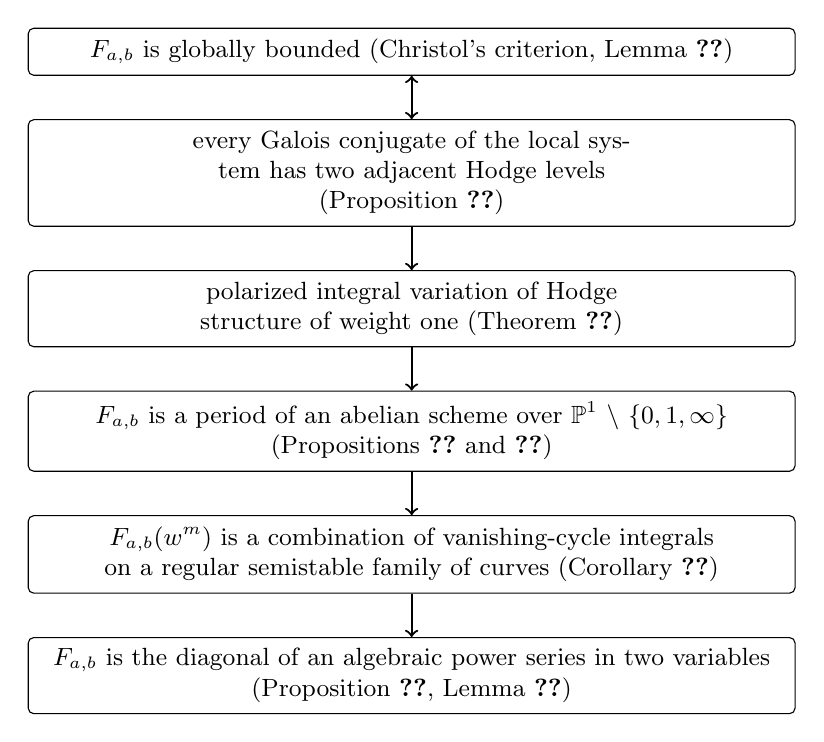
\begin{tikzpicture}[node distance=5.5mm,
  box/.style={draw, rounded corners=2pt, align=center, inner sep=4pt, font=\small, text width=0.78\textwidth}]
\node[box] (gb) {$\Fab$ is globally bounded (Christol's criterion, Lemma~\ref{lem:christol})};
\node[box, below=of gb] (two) {every Galois conjugate of the local system has two adjacent Hodge levels\\ (Proposition~\ref{prop:twolevel})};
\node[box, below=of two] (wt) {polarized integral variation of Hodge structure of weight one (Theorem~\ref{thm:wt1})};
\node[box, below=of wt] (ab) {$\Fab$ is a period of an abelian scheme over $\PP^1\setminus\{0,1,\infty\}$\\ (Propositions~\ref{prop:abelian} and~\ref{prop:period})};
\node[box, below=of ab] (cu) {$\Fab(w^m)$ is a combination of vanishing-cycle integrals on a regular semistable family of curves (Corollary~\ref{cor:vanishing})};
\node[box, below=of cu] (di) {$\Fab$ is the diagonal of an algebraic power series in two variables\\ (Proposition~\ref{prop:node}, Lemma~\ref{lem:closure})};
\draw[<->, thick] (gb) -- (two);
\draw[->, thick] (two) -- (wt);
\draw[->, thick] (wt) -- (ab);
\draw[->, thick] (ab) -- (cu);
\draw[->, thick] (cu) -- (di);
\end{tikzpicture}
\caption{The structure of the proof of Theorem~\ref{thm:A}.}\label{fig:strategy}
\end{figure}

\subsection{Related work}
\emph{Diagonals and periods.} \citet{Christol1985} and \citet{Deligne1984} connected diagonals of rational functions with integrals over vanishing cycles, and \citet[Theorem~12]{Christol1990} turned this into the sufficient condition recalled above. \citet[\S4.2]{Christol2015} explains the role of the duality between the monodromy weight filtration and the pole-order filtration. \citet{BostanEtAl2013} used these ideas to show that many integrals from the Ising model and many solutions of Calabi--Yau equations are diagonals, and discussed $H$ as a test case of intermediate weight. \citet{HarderKramerMiller2026} relate the minimal number of variables in a diagonal representation to the nilpotence of the local monodromy. Their Lemma~3.2 identifies diagonals of algebraic series in $n+1$ variables with diagonals of rational functions in $n+2$ variables; we use it to pass from two algebraic to three rational variables. \citet{HassaniMaillardZenine2025} formulate conjectures on the minimal number of variables in terms of the powers of the logarithm in the formal solutions.

\emph{Global boundedness and algebraicity.} \citet{Christol1987} characterized the globally bounded hypergeometric series with rational parameters by an interlacing condition over all Galois conjugates of the parameters. \citet{BeukersHeckman1989} gave the analogous criterion for finite monodromy, hence for algebraicity, and determined the monodromy groups. \citet{FurnsinnYurkevich2024} extended the algebraicity criterion to arbitrary parameters, and \citet{CarusoFurnsinn2026a,CarusoFurnsinn2026b} implemented these criteria and related arithmetic invariants.

\emph{Hypergeometric diagonals.} \citet{AbdelazizKoutschanMaillard2020} represented their two series, and the one-parameter family of Proposition~\ref{prop:D}(b), as diagonals of algebraic functions in three variables. Using the algorithm of \citet{DenefLipshitz1987}, they also wrote down rational functions in six variables with these diagonals, and they settled further ${}_3F_2$ and ${}_4F_3$ examples. \citet{BostanYurkevich2022} determined the hypergeometric series that arise as diagonals of products of powers of $1-x_1-\dots-x_n$. Proposition~\ref{prop:D}(a) shows that the two series of Abdelaziz, Koutschan and Maillard are Hadamard products of two algebraic series, and Proposition~\ref{prop:D}(b) represents their one-parameter family with two algebraic variables.

\emph{Hodge theory of hypergeometric local systems.} Hypergeometric local systems are rigid, and \citet{Katz1996} showed that rigid local systems with quasi-unipotent local monodromy are of geometric origin. \citet[Proposition~2.6]{Fedorov2018} shows that a hypergeometric connection with real parameters underlies a polarizable complex variation of Hodge structure, unique up to a shift of the grading; for existence he uses \citet[Corollary~8.1]{Simpson1990} and \citet[Theorem~2.4.1]{DettweilerSabbah2013}, and for uniqueness \citet[Proposition~1.13(i)]{Deligne1987}. He also computes the Hodge numbers \citep[Theorem~1]{Fedorov2018}. This formula is the main input of Proposition~\ref{prop:twolevel}. Restriction of scalars and diagonals are not considered there.

\emph{Geometric realizations.} The Euler integral realizes ${}_nF_{n-1}$ as a period of a family of varieties of relative dimension $n-1$; see \citet[\S4.3]{Christol2015} for ${}_3F_2$ and \citet{KellyVoight2024} for the resulting hypergeometric motives. For ${}_2F_1$ the realization is by curves, and \citet{Archinard2003} constructed the corresponding abelian varieties explicitly. Our weight-one realization of ${}_3F_2$ comes instead from the equivalence of \citet[4.4.3]{Deligne1971} between abelian schemes and polarizable variations of Hodge structure of weight one, proved in detail by \citet[Theorem~7.13]{Milne2013}. Over a point, the passage from the weight-two Hodge structure of the Euler realization to weight one is a half twist \citep{vanGeemen2001,vanGeemenIzadi2002}. Periods of degenerating abelian varieties over locally invariant cycles were studied by \citet{Andre1989} in connection with $G$-functions.

To our knowledge, no proof that $H$ is a diagonal has appeared. In the examples of series $\Fab$ with $b\notin\Z$ that we know to be diagonals, including those of Proposition~\ref{prop:D}, the representation is explicit. For $H$ none is known, and the search of Appendix~\ref{app:search} found none of the simplest kinds. Each ingredient of our proof is classical. What appears to be new is the equivalence of Proposition~\ref{prop:twolevel} and its use, through a realization of weight one, to bring Christol's minimum-weight principle to bear.

\subsection{Organization}
Section~\ref{sec:prelim} collects the facts we need on algebraic power series, hypergeometric local systems, global boundedness and variations of Hodge structure. Sections~\ref{sec:twolevel}--\ref{sec:node} carry out steps (1)--(5), and Theorem~\ref{thm:A} is proved in \S\ref{subsec:proofA}. Section~\ref{sec:examples} treats the examples and proves Corollaries~\ref{cor:B} and~\ref{cor:C} and Proposition~\ref{prop:D}. Section~\ref{sec:remarks} contains concluding remarks. Appendix~\ref{app:euler} gives an independent computational check of the Hodge numbers, Appendix~\ref{app:certificates} describes the accompanying computations, and Appendix~\ref{app:search} reports a search for explicit representations of $H$.

\subsection*{Notation and conventions}
We write $\e(t)=e^{2\pi it}$ and $U=\PP^1\setminus\{0,1,\infty\}$, a scheme over $\Q$; base change to a field $F$ is denoted by $U_F$, and $U(\C)$ carries its analytic topology. We put $\theta=x\,\frac{d}{dx}$. Local systems are on $U(\C)$ unless stated otherwise. The local monodromy around $0$ of any local system on $U(\C)$ is denoted by $T_0$; on solutions of a differential equation it acts by analytic continuation. For $t\in\R$, $\{t\}\in[0,1)$ is the fractional part. The letter $k$ always denotes an element of $(\Z/N\Z)^\times$, where $N$ is a common denominator of the parameters. Complex conjugation is denoted by a bar, and $X^*=\overline X^{\,T}$ for a complex matrix $X$. For a field $F$ and variables $u_1,\dots,u_n$, $\alg F{u_1,\dots,u_n}$ is the ring of power series in $F[[u_1,\dots,u_n]]$ that are algebraic over $F(u_1,\dots,u_n)$. The Hadamard product of $f=\sum a_nx^n$ and $g=\sum b_nx^n$ is $f\star g=\sum a_nb_nx^n$; it equals $\Diag\big(f(u)g(v)\big)$.

%======================================================================
\section{Preliminaries}\label{sec:prelim}
%======================================================================

\subsection{Algebraic power series and diagonals}\label{subsec:alg}
Let $F$ be a field of characteristic $0$. The ring $\alg F{u_1,\dots,u_n}$ is the henselization of the local ring of $\A^n_F$ at the origin. More generally, let $\cO$ be the local ring of a smooth $F$-variety of dimension $n$ at an $F$-rational point, and let $u_1,\dots,u_n$ be a regular system of parameters of its henselization $\cO^h$. Then $\cO^h=\alg F{u_1,\dots,u_n}$ inside the completion $\widehat\cO=F[[u_1,\dots,u_n]]$; see \citet[\S\S1 and~5]{Artin1969} and \citet[\S18]{EGAIV4}. The ring $\alg F{u_1,\dots,u_n}$ is closed under partial derivatives and under the specializations $u_i=0$. If $F\subset\C$, its elements converge in a neighbourhood of the origin.

For $g=\sum_{j,l\ge0}g_{j,l}u^jv^l\in F[[u,v]]$ we put $\Diag(g)(w)=\sum_{n\ge0}g_{n,n}w^n$. The following closure properties are elementary; we include proofs because we need them for two-variable algebraic series and over number fields.

\begin{lemma}\label{lem:closure}
Let $F\subset\C$ be a number field.
\begin{enumerate}[label=\textup{(\alph*)},leftmargin=2em]
\item Let $\varphi_1,\dots,\varphi_r\in F[[w]]$ and $z_1,\dots,z_r\in\C$. If $\sum_iz_i\varphi_i$ lies in $F[[w]]$, then it equals $\sum_ic_i\varphi_i$ for some $c_1,\dots,c_r\in F$.
\item If $g\in\alg F{u,v}$ and $\Diag(g)\in\Q[[w]]$, then $\Diag(g)=\Diag(g')$ for some $g'\in\alg\Q{u,v}$.
\item If $g\in\alg\Q{u,v}$ and $\Diag(g)=w^\nu\varphi(w)$ with $\nu\ge0$ and $\varphi\in\Q[[w]]$, then $\varphi=\Diag(g')$ for some $g'\in\alg\Q{u,v}$.
\item If $g\in\alg\Q{u,v}$ and $\Diag(g)(w)=\varphi(w^m)$ with $m\ge1$ and $\varphi\in\Q[[w]]$, then $\varphi=\Diag(g')$ for some $g'\in\alg\Q{u,v}$.
\end{enumerate}
\end{lemma}

\begin{proof}
(a) After renumbering, $\varphi_1,\dots,\varphi_s$ form a basis of the $F$-span of the $\varphi_i$. Then $\sum_iz_i\varphi_i=\sum_{j\le s}y_j\varphi_j$ with $y_j\in\C$. Since $\varphi_1,\dots,\varphi_s$ are linearly independent over $F$, there are exponents $n_1,\dots,n_s$ such that the $s\times s$ matrix formed by the coefficients of $w^{n_l}$ in $\varphi_j$ is invertible. Comparing the coefficients of $w^{n_1},\dots,w^{n_s}$, which lie in $F$ on both sides, gives $y_j\in F$.

(b) Replacing $F$ by its Galois closure, we may assume that $F$ is Galois over $\Q$, with group $\Gamma$. For $\sigma\in\Gamma$ let $\sigma(g)$ be the series obtained by applying $\sigma$ to the coefficients of $g$. It is algebraic, since it satisfies the conjugate polynomial equation, and $\Diag(\sigma(g))=\sigma(\Diag(g))=\Diag(g)$. The series $g'=|\Gamma|^{-1}\sum_{\sigma\in\Gamma}\sigma(g)$ has rational coefficients, is algebraic over $F(u,v)$ and hence over $\Q(u,v)$, and satisfies $\Diag(g')=\Diag(g)$.

(c) Put $g'=\sum_{j,l\ge\nu}g_{j,l}u^{j-\nu}v^{l-\nu}$, so that $\Diag(g')=\varphi$. The series $g_j(v)=\sum_lg_{j,l}v^l=\frac1{j!}\,\partial_u^jg(0,v)$ and $g^l(u)=\sum_jg_{j,l}u^j$ are algebraic. Hence so is
\[
(uv)^\nu g'=g-\sum_{j<\nu}u^jg_j(v)-\sum_{l<\nu}v^lg^l(u)+\sum_{j,l<\nu}g_{j,l}u^jv^l ,
\]
and therefore so is $g'$.

(d) Put $g'=\sum_{j,l\ge0}g_{mj,ml}u^jv^l\in\Q[[u,v]]$, so that $\Diag(g')=\varphi$. Then
\[
g'(u^m,v^m)=\frac1{m^2}\sum_{j,l=0}^{m-1}g\big(\e(j/m)u,\e(l/m)v\big)
\]
is algebraic over $\Q(\e(1/m))(u,v)$, hence over $\Q(u,v)$, hence over the subfield $\Q(u^m,v^m)$, over which $\Q(u,v)$ is finite. Renaming $u^m,v^m$ as $u,v$ shows that $g'$ is algebraic.
\end{proof}

\begin{lemma}[{\citealp[Lemma~3.2]{HarderKramerMiller2026}}]\label{lem:HKM}
Let $F$ be a field of characteristic $0$, let $n\ge0$ and let $f\in F[[x]]$. Then $f$ is the diagonal of an algebraic power series in $n+1$ variables over $F$ if and only if it is the diagonal of a rational function in $n+2$ variables over $F$ that is regular at the origin.
\end{lemma}

The proof of Lemma~\ref{lem:HKM} rests on \citet[Theorem~6.2 and Remark~6.4]{DenefLipshitz1987}. Applied directly, the theorem of Denef and Lipshitz gives $2(n+1)$ rational variables.

\begin{theorem}[{\citealp{Polya1922,Furstenberg1967}}]\label{thm:furst}
Let $F$ be a field of characteristic $0$. The diagonal of a rational function in two variables over $F$ that is regular at the origin is algebraic over $F(x)$. Conversely, every power series in $F[[x]]$ that is algebraic over $F(x)$ is such a diagonal.
\end{theorem}

\subsection{Hypergeometric local systems}\label{subsec:hyp}
The series $\Fab$ is annihilated by the hypergeometric operator
\begin{equation}\label{eq:L}
L_{a,b}=\theta^2(\theta+b-1)-x(\theta+a_1)(\theta+a_2)(\theta+a_3).
\end{equation}
Its singular points are $0$, $1$ and $\infty$, with local exponents $0,0,1-b$ at $0$, with $a_1,a_2,a_3$ at $\infty$, and with $0,1,b+1-a_1-a_2-a_3$ at $1$. Let $\Sab$ denote the local system of solutions of $L_{a,b}$ on $U(\C)$. Put
\[
P_a(t)=\prod_{j=1}^3\big(t-\e(a_j)\big),\qquad P_b(t)=(t-1)^2\big(t-\e(b)\big),
\]
and let $A$ and $B$ be the companion matrices of $P_a$ and $P_b$.

\begin{lemma}[{Levelt; see \citealp[Proposition~3.3 and Theorem~3.5]{BeukersHeckman1989}}]\label{lem:levelt}
Assume \eqref{eq:NR}. Then $\Sab$ is irreducible. For a suitable basis of a fibre, and suitable loops around $0$, $1$ and $\infty$ whose product is trivial, the local monodromy matrices are
\[
T_0=B^{-1},\qquad T_1=A^{-1}B,\qquad T_\infty=A,\qquad T_\infty T_1T_0=1 ,
\]
and $T_1-1$ has rank one. In particular, $\Sab$ depends up to isomorphism only on $P_a$ and $P_b$, that is, on $a$ and $b$ modulo $\Z$.
\end{lemma}

The eigenvalues of $T_0=B^{-1}$ are $1,1,\e(-b)$, in accordance with the local exponents $0,0,1-b$.

\begin{lemma}\label{lem:local0}
Assume \eqref{eq:NR}, and let $d$ be the denominator of $b$.
\begin{enumerate}[label=\textup{(\roman*)},leftmargin=2em]
\item Near $0$ the solutions of $L_{a,b}$ are spanned by $\Fab$, by a solution $Y=\Fab\log x+G$ with $G\in x\,\Q[[x]]$, and by a solution in $x^{1-b}\,\Q[[x]]$.
\item We have $T_0\Fab=\Fab$ and $(T_0^m-1)Y=2\pi i\,m\,\Fab$ for every $m\ge1$.
\item The minimal polynomial of $T_0$ is $(t-1)^2(t-\e(-b))$. The operator $T_0^d$ is unipotent, with $(T_0^d-1)^2=0$ and $\rank(T_0^d-1)=1$.
\item The series $\Fab$ is transcendental over $\Q(x)$.
\end{enumerate}
\end{lemma}

\begin{proof}
(i) The indicial polynomial of $L_{a,b}$ at $0$ is $\theta^2(\theta+b-1)$, with roots $0,0,1-b$, and $1-b\notin\Z$. The statement follows from the Frobenius method. (ii) This follows from (i), since $\log x$ increases by $2\pi i$ under $T_0$. (iii) A companion matrix is non-derogatory, that is, its minimal polynomial equals its characteristic polynomial, and the same holds for its inverse. Hence $T_0$ has a single Jordan block of size two for the eigenvalue $1$, and the simple eigenvalue $\e(-b)$. Its $d$-th power has a single Jordan block of size two for the eigenvalue $1$ and the further eigenvalue $\e(-db)=1$. (iv) If $\Fab$ were algebraic, its analytic continuations would span a nonzero sub-local system of $\Sab$ with finite monodromy. By irreducibility this would be all of $\Sab$, contradicting (iii).
\end{proof}

\subsection{Global boundedness}
For $t\in\R$ let $\langle t\rangle\in(0,1]$ denote the representative of $t$ modulo $\Z$ in $(0,1]$.

\begin{lemma}[{\citealp[Propositions~1 and~1bis]{Christol1987}; see also \citealp{FurnsinnYurkevich2024}}]\label{lem:christol}
Let $a_1,a_2,a_3\in\Q\setminus\Z$ and $b_1,b_2\in(\Q\setminus\Z)\cup\{1\}$ with $a_i-b_j\notin\Z$ for all $i,j$. Let $N$ be a common denominator of the parameters, and put $b_3=1$. Then ${}_3F_2(a_1,a_2,a_3;b_1,b_2;x)$ is globally bounded if and only if, for every $k\in(\Z/N\Z)^\times$ and every $t\in(0,1)$,
\[
\#\{i:\langle ka_i\rangle\le t\}\ \ge\ \#\{j:\langle kb_j\rangle\le t\}.
\]
\end{lemma}

\subsection{Complex variations of Hodge structure}
We recall the notion of a complex variation of Hodge structure; see \citet[\S1]{Deligne1987} and \citet{Simpson1988}. For a complex manifold $M$ we write $\cE^{p,q}_M$ for the sheaf of smooth forms of type $(p,q)$ and $\cE^0_M$ for the sheaf of smooth functions.

\begin{definition}\label{def:cvhs}
Let $M$ be a complex manifold and $\cS$ a local system of finite-dimensional complex vector spaces on $M$, with flat connection $\nabla$ on the smooth bundle $\cS\otimes\cE^0_M$. A \emph{complex variation of Hodge structure} on $\cS$ is a decomposition $\cS\otimes\cE^0_M=\bigoplus_{p\in\Z}\cS^p$ into smooth subbundles such that
\begin{equation}\label{eq:griffiths}
\nabla(\cS^p)\subset\cE^{1,0}_M(\cS^p\oplus\cS^{p-1})\oplus\cE^{0,1}_M(\cS^p\oplus\cS^{p+1})\qquad\text{for all }p .
\end{equation}
The \emph{Hodge numbers} are $h^p=\rank\cS^p$. The variation is \emph{polarized} by a flat hermitian form $Q$ on $\cS$ if the subbundles $\cS^p$ are mutually orthogonal for $Q$ and $(-1)^pQ$ is positive definite on $\cS^p$ for every $p$. It is \emph{polarizable} if such a form exists.
\end{definition}

By \eqref{eq:griffiths}, the bundle $\bigoplus_{q\ge p}\cS^q$ is a holomorphic subbundle of $\cS\otimes\cO_M$ for every $p$. In particular, if only two degrees $p$ and $p-1$ occur, then $\cS^p$ is a holomorphic subbundle, and $\cS^{p-1}$ is stable under the $(1,0)$-part of $\nabla$. In this case we call $\cS^p$ the \emph{top piece} and $\cS^{p-1}$ the \emph{bottom piece}, and we say that the variation has \emph{two adjacent Hodge levels}.

\begin{theorem}[{\citealp[Proposition~2.6 and Theorem~1]{Fedorov2018}}]\label{thm:fedorov}
Let $0\le\alpha_1\le\alpha_2\le\alpha_3<1$ and $0\le\beta_1\le\beta_2\le\beta_3<1$ be real numbers with $\alpha_i\ne\beta_j$ for all $i,j$. The connection on $U$ defined by the operator $\prod_j(\theta-\alpha_j)-x\prod_j(\theta-\beta_j)$ underlies a polarizable complex variation of Hodge structure, which is unique up to a shift of the grading. Up to such a shift, its Hodge numbers are
\[
h^p=\#\{l:\rho(l)=p\},\qquad\text{where }\rho(l)=\#\{j:\alpha_j<\beta_l\}-l\quad(l=1,2,3).
\]
\end{theorem}

For the existence statement Fedorov refers to \citet[Corollary~8.1]{Simpson1990} and \citet[Theorem~2.4.1]{DettweilerSabbah2013}, and for uniqueness to \citet[Proposition~1.13(i)]{Deligne1987}. His theorem holds in every rank; we need it only in rank three.

\begin{remark}\label{rem:dual}
The dual of a polarized complex variation of Hodge structure is again one, with the Hodge numbers in reverse order. The local system of solutions of a differential operator is dual to the local system of horizontal sections of the corresponding connection. Hence it does not matter, for the property of having two adjacent Hodge levels, whether Theorem~\ref{thm:fedorov} is read on the connection or on its solutions.
\end{remark}

\begin{lemma}\label{lem:conj}
Let $(\cS,\bigoplus_p\cS^p,Q)$ be a polarized complex variation of Hodge structure on $M$, and let $\overline{\cS}$ be the complex conjugate local system. Put $\overline{\cS}^{\,q}=\overline{\cS^{-q}}$ and $\overline Q(\bar s,\bar s')=\overline{Q(s,s')}$. Then $(\overline{\cS},\bigoplus_q\overline{\cS}^{\,q},\overline Q)$ is a polarized complex variation of Hodge structure. In particular, if $\cS$ has two adjacent Hodge levels, then so has $\overline{\cS}$; the complex conjugate of the bottom piece of $\cS$ is the top piece of $\overline{\cS}$, and it is a holomorphic subbundle of $\overline{\cS}\otimes\cO_M$.
\end{lemma}

\begin{proof}
The flat connection of $\overline{\cS}$ is given by $\overline\nabla(\bar s)=\overline{\nabla s}$, and complex conjugation exchanges $\cE^{1,0}_M$ and $\cE^{0,1}_M$. Conjugating \eqref{eq:griffiths} gives
\[
\overline\nabla\big(\overline{\cS^p}\big)\subset\cE^{0,1}_M\big(\overline{\cS^p}\oplus\overline{\cS^{p-1}}\big)\oplus\cE^{1,0}_M\big(\overline{\cS^p}\oplus\overline{\cS^{p+1}}\big),
\]
which is \eqref{eq:griffiths} for the decomposition $\overline{\cS}^{\,q}=\overline{\cS^{-q}}$. The form $\overline Q$ is flat and hermitian, the subbundles $\overline{\cS}^{\,q}$ are mutually orthogonal, and $\overline Q$ has on $\overline{\cS}^{\,q}$ the sign of $Q$ on $\cS^{-q}$, which is $(-1)^q$. If $\cS=\cS^p\oplus\cS^{p-1}$, then the top piece of $\overline{\cS}$ is $\overline{\cS}^{\,1-p}=\overline{\cS^{p-1}}$, and it is holomorphic by the remark following Definition~\ref{def:cvhs}.
\end{proof}

\subsection{Weight one and abelian schemes}
\begin{definition}\label{def:zvhs}
Let $M$ be a complex manifold. A \emph{polarized variation of Hodge structure of type $\{(1,0),(0,1)\}$} on $M$ consists of a local system $V_\Z$ of free $\Z$-modules of finite rank, a holomorphic subbundle $F^1\subset V_\C\otimes\cO_M$ such that $V_\C\otimes\cE^0_M=F^1\oplus\overline{F^1}$, and a flat alternating form $\psi:V_\Z\times V_\Z\to\Z$ such that $\psi(F^1,F^1)=0$ and $i\,\psi(v,\bar v)>0$ for all nonzero $v\in F^1$. Here $V_\C=V_\Z\otimes\C$, and $\psi$ is extended bilinearly.
\end{definition}

Griffiths transversality is automatic for this type. The Tate twist $V_\Z(1)$ has type $\{(-1,0),(0,-1)\}$ and the same underlying local system.

\begin{theorem}[{\citealp[4.4.3]{Deligne1971}; \citealp[Theorem~7.13]{Milne2013}}]\label{thm:deligne}
Let $S$ be a smooth scheme of finite type over $\C$. The functor $(f:\cA\to S)\mapsto R_1f_*\Z$ is an equivalence between the category of abelian schemes over $S$ and the category of polarizable variations of Hodge structure of type $\{(-1,0),(0,-1)\}$ on $S(\C)$ whose underlying local system is torsion-free.
\end{theorem}

In the literature the statement is phrased either in terms of the homology $R_1f_*\Z$, as here, or in terms of the cohomology $R^1f_*\Z$ and the type $\{(1,0),(0,1)\}$. With either convention, a polarization identifies $V_\Q$ with its dual. Hence the abelian scheme $f:\cA\to S$ attached to $V_\Z(1)$ satisfies $R_1f_*\Q\cong V_\Q$, which is all we use.

%======================================================================
\section{Two Hodge levels and global boundedness}\label{sec:twolevel}
%======================================================================

In this section we assume \eqref{eq:NR}. Let $N$ be the common denominator of $a_1,a_2,a_3,b$. For $k\in(\Z/N\Z)^\times$ the pair $(ka,kb)$ again satisfies \eqref{eq:NR}, and by Lemma~\ref{lem:levelt} the local system $\cS_{ka,kb}$ depends only on the class of $k$ modulo $N$. We write
\[
\ak1\le\ak2\le\ak3\qquad\text{and}\qquad\bk=\{kb\}
\]
for the fractional parts $\{ka_1\},\{ka_2\},\{ka_3\}$ in increasing order and for the fractional part of $kb$. All four numbers lie in the open interval $(0,1)$, and $\bk\ne\ak i$ for all $i$.

\begin{proposition}\label{prop:twolevel}
Assume \eqref{eq:NR} and let $k\in(\Z/N\Z)^\times$. The local system $\cS_{ka,kb}$ underlies a polarizable complex variation of Hodge structure, unique up to a shift of the grading. For the operator $L_{ka,kb}$, the formula of Theorem~\ref{thm:fedorov} gives the following nonzero Hodge numbers, listed from the highest degree to the lowest:
\[
\begin{array}{ll}
(1,1,1) & \text{if } \bk<\ak1,\\[1pt]
(1,2) & \text{if } \ak1<\bk<\ak2,\\[1pt]
(2,1) & \text{if } \ak2<\bk<\ak3,\\[1pt]
(1,1,1) & \text{if } \ak3<\bk.
\end{array}
\]
In particular, the variation on $\cS_{ka,kb}$ has two adjacent Hodge levels if and only if $\ak1<\bk<\ak3$. Moreover, the series $\Fab$ is globally bounded if and only if $\ak1<\bk<\ak3$ for every $k\in(\Z/N\Z)^\times$.
\end{proposition}

\begin{proof}
We have $\theta^2(\theta+kb-1)=\prod_j(\theta-\alpha_j)$ with $\alpha=(0,0,1-kb)$, and $\prod_j(\theta+ka_j)=\prod_j(\theta-\beta_j)$ with $\beta_j=-ka_j$. By Lemma~\ref{lem:levelt} we may replace these parameters by their fractional parts without changing the local system. In the notation of Theorem~\ref{thm:fedorov} we may therefore take
\[
\alpha=(0,0,1-\bk),\qquad\beta=(1-\ak3,\,1-\ak2,\,1-\ak1),
\]
which are sorted and satisfy $\alpha_i\ne\beta_j$ for all $i,j$. Existence and uniqueness of the variation follow from Theorem~\ref{thm:fedorov} and Remark~\ref{rem:dual}. For $l=1,2,3$ we have $\#\{j:\alpha_j<\beta_l\}=2+[\,1-\bk<\beta_l\,]$, where $[\,\cdot\,]$ equals $1$ if the condition holds and $0$ otherwise, and $1-\bk<1-\ak{4-l}$ holds exactly when $\ak{4-l}<\bk$. Hence
\[
\big(\rho(1),\rho(2),\rho(3)\big)=\big(1+[\ak3<\bk],\ [\ak2<\bk],\ -1+[\ak1<\bk]\big).
\]
The four cases of the proposition correspond to $0$, $1$, $2$ or $3$ of the numbers $\ak i$ being smaller than $\bk$, and give $\rho=(1,0,-1)$, $(1,0,0)$, $(1,1,0)$ and $(2,1,0)$.

For the last statement we apply Lemma~\ref{lem:christol} with $(b_1,b_2,b_3)=(b,1,1)$. Here $\langle ka_i\rangle=\{ka_i\}$ and $\langle kb\rangle=\bk$, while $\langle kb_2\rangle=\langle kb_3\rangle=1$. The condition of the lemma at $k$ therefore reads $\#\{i:\ak i\le t\}\ge[\bk\le t]$ for all $t\in(0,1)$, which is equivalent to $\ak1<\bk$. So $\Fab$ is globally bounded if and only if $\ak1<\bk$ for all $k$. Since $\{-t\}=1-\{t\}$ for $t\notin\Z$, replacing $k$ by $-k$ replaces $\ak1$ by $1-\ak3$ and $\bk$ by $1-\bk$. The condition at $-k$ is therefore $\bk<\ak3$. Hence the conditions for all $k$ together are equivalent to $\ak1<\bk<\ak3$ for all $k$.
\end{proof}

\begin{remark}
Below we use only whether a conjugate has two adjacent Hodge levels. Which of the patterns $(1,2)$ and $(2,1)$ belongs to $\cS_{ka,kb}$ and which to its dual depends on the convention discussed in Remark~\ref{rem:dual}, and plays no role. Appendix~\ref{app:euler} contains an independent check of the Hodge numbers of Proposition~\ref{prop:twolevel}, obtained by counting square-integrable holomorphic $2$-forms on the surfaces of the Euler integral.
\end{remark}

%======================================================================
\section{A polarized variation of Hodge structure of weight one}\label{sec:wt1}
%======================================================================

Throughout this section $(a,b)$ satisfies \eqref{eq:NR} and $\Fab$ is globally bounded. Let $N$ be the common denominator of the parameters. Put $\zeta_N=\e(1/N)$ and $K=\Q(\zeta_N)\subset\C$, with ring of integers $\cO_K=\Z[\zeta_N]$. Let $K^+=K\cap\R$, and for $k\in(\Z/N\Z)^\times$ let $\sigma_k$ be the automorphism of $K$ with $\sigma_k(\zeta_N)=\zeta_N^k$. Complex conjugation preserves $K$ and equals $\sigma_{-1}$.

\begin{lemma}\label{lem:CM}
We have $N\ge3$. Consequently $K$ is a CM field of degree $\varphi(N)$ with maximal totally real subfield $K^+$, complex conjugation commutes with every $\sigma_k$, and $\sigma_k\ne\sigma_{-k}$ for all $k$.
\end{lemma}

\begin{proof}
If $N\le2$, then the non-integers $a_1,a_2,a_3,b$ all lie in $\frac12+\Z$, so that $a_i-b\in\Z$, contradicting \eqref{eq:NR}. The remaining statements hold for every cyclotomic field $\Q(\zeta_N)$ with $N\ge3$.
\end{proof}

We fix a nonzero element $\xi_0\in K$ with $\overline{\xi_0}=-\xi_0$, for instance $\xi_0=\zeta_N-\zeta_N^{-1}$. Every $\xi\in K$ with $\bar\xi=-\xi$ is of the form $\lambda\xi_0$ with $\lambda\in K^+$.

\subsection{The cyclotomic lattice}
The coefficients of $P_a$ and $P_b$ are symmetric functions of $N$-th roots of unity, so $A$ and $B$ have entries in $\cO_K$. Their determinants $\e(a_1+a_2+a_3)$ and $\e(b)$ are roots of unity, so $A,B\in\mathrm{GL}_3(\cO_K)$. Let $\Lambda$ be the local system on $U(\C)$ with fibre $\cO_K^3$ and with the monodromy matrices $T_0=B^{-1}$, $T_1=A^{-1}B$, $T_\infty=A$ of Lemma~\ref{lem:levelt}. Let $V_\Z$ be $\Lambda$ viewed as a local system of free $\Z$-modules of rank $3\varphi(N)$, and put $V_\Q=V_\Z\otimes\Q$ and $V_\C=V_\Z\otimes\C$. The fibre of $V_\Q$ is $K^3$, and the isomorphism $K\otimes_\Q\C\cong\C^{\varphi(N)}$, $x\otimes1\mapsto(\sigma_k(x))_k$, gives a decomposition
\begin{equation}\label{eq:split}
V_\C=\bigoplus_{k\in(\Z/N\Z)^\times}\cS_k .
\end{equation}
Here $\cS_k$ has fibre $\C^3$ and monodromy matrices $\sigma_k(B)^{-1}$, $\sigma_k(A)^{-1}\sigma_k(B)$, $\sigma_k(A)$. Since $\sigma_k(A)$ and $\sigma_k(B)$ are the companion matrices of $P_{ka}$ and $P_{kb}$, Lemma~\ref{lem:levelt} gives $\cS_k\cong\cS_{ka,kb}$; in particular $\cS_1\cong\Sab$. We write elements of $V_\C$ as $X=(X_k)_k$ with $X_k\in\cS_k$. Complex conjugation on $V_\C$ with respect to $V_\Q$ is then given by
\begin{equation}\label{eq:conj}
(\overline X)_k=\overline{X_{-k}} .
\end{equation}
It maps $\cS_k$ antilinearly onto $\cS_{-k}$, compatibly with the flat structures, and so identifies $\cS_{-k}$ with the complex conjugate local system $\overline{\cS_k}$.

\subsection{Invariant hermitian forms}
\begin{lemma}\label{lem:herm}
There is a matrix $h\in M_3(K)$ with $h^*=h$ and $\det h\ne0$ such that $A^*hA=h$ and $B^*hB=h$. It is unique up to multiplication by an element of $(K^+)^\times$. For every $k$, the form
\[
\langle X,X'\rangle_k=X^*\sigma_k(h)X'
\]
is a flat nondegenerate hermitian form on $\cS_k$, and every flat hermitian form on $\cS_k$ is a real multiple of it.
\end{lemma}

\begin{proof}
The equations $A^*XA=X$ and $B^*XB=X$ form a system of linear equations over $K$ in the entries of a $3\times3$ matrix $X$. By Proposition~\ref{prop:twolevel}, the local system $\cS_1$ carries a polarized complex variation of Hodge structure, hence a flat nondegenerate hermitian form. Its Gram matrix in the basis of Lemma~\ref{lem:levelt} is a nonzero complex solution of the system. A system of linear equations over $K$ that has a nonzero solution over $\C$ has a nonzero solution over $K$; let $X$ be one. Then $X^*$ is also a solution. If $X+X^*\ne0$ we put $h=X+X^*$, and otherwise $h=\xi_0X$, which is hermitian because $X^*=-X$. The relation $A^*hA=h$ gives $hAv=(A^*)^{-1}hv$, and similarly for $B$, so the kernel of $h$ is stable under the monodromy; it is zero because $\cS_1$ is irreducible. If $h'$ is a second matrix with these properties, then $h^{-1}h'$ commutes with $A$ and $B$ and is therefore a scalar $\lambda\in K$, by irreducibility, and $\lambda\in K^+$ because $h$ and $h'$ are hermitian. Applying $\sigma_k$, which commutes with complex conjugation, shows that $\sigma_k(h)$ is hermitian, nondegenerate and invariant under $\sigma_k(A)$ and $\sigma_k(B)$. Finally, a flat hermitian form on the irreducible local system $\cS_k$ is zero or nondegenerate, because its kernel is a sub-local system. Two flat nondegenerate hermitian forms differ by an automorphism of $\cS_k$, that is, by a scalar, and this scalar is real.
\end{proof}

\subsection{The variation of weight one}
\begin{theorem}\label{thm:wt1}
Assume \eqref{eq:NR} and that $\Fab$ is globally bounded. Then there are a holomorphic subbundle $F^1\subset V_\C\otimes\cO_{U(\C)}$ of rank $\frac32\varphi(N)$ and an element $\lambda\in(K^+)^\times$ such that $V_\Z$, $F^1$ and the form
\[
\psi(x,y)=\Tr_{K/\Q}\big(\lambda\,\xi_0\,x^*hy\big)\qquad(x,y\in K^3)
\]
constitute a polarized variation of Hodge structure of type $\{(1,0),(0,1)\}$ on $U(\C)$.
\end{theorem}

\begin{proof}
\emph{Step 1: the Hodge decomposition.} Let $\Phi\subset(\Z/N\Z)^\times$ be a set of representatives modulo $\pm1$; by Lemma~\ref{lem:CM} it has $\frac12\varphi(N)$ elements. For $k\in\Phi$ we choose on $\cS_k\cong\cS_{ka,kb}$ a polarized complex variation of Hodge structure, as in Proposition~\ref{prop:twolevel}. Since $\Fab$ is globally bounded, it has two adjacent Hodge levels; let $\cS_k^{\tp}$ and $\cS_k^{\bt}$ be its top and bottom pieces. For $k\in-\Phi$ we have $\cS_k=\overline{\cS_{-k}}$, and we give $\cS_k$ the conjugate variation of Lemma~\ref{lem:conj}. Its top and bottom pieces are
\[
\cS_k^{\tp}=\overline{\cS_{-k}^{\bt}}\qquad\text{and}\qquad\cS_k^{\bt}=\overline{\cS_{-k}^{\tp}} .
\]
For every $k$, the subbundle $\cS_k^{\tp}$ of $\cS_k\otimes\cO$ is holomorphic, by the remark following Definition~\ref{def:cvhs} and by Lemma~\ref{lem:conj}. We put
\[
F^1=\bigoplus_k\cS_k^{\tp} .
\]
By construction and by \eqref{eq:conj}, complex conjugation maps $\cS_k^{\tp}$ onto $\cS_{-k}^{\bt}$ for every $k$. Hence $\overline{F^1}=\bigoplus_k\cS_k^{\bt}$ and $V_\C\otimes\cE^0=F^1\oplus\overline{F^1}$. The rank of $F^1$ is $\sum_{k\in\Phi}(\rank\cS_k^{\tp}+\rank\cS_k^{\bt})=\frac32\varphi(N)$.

\emph{Step 2: orthogonality and signs.} Let $Q_k$ be the polarization of the variation chosen on $\cS_k$. By Lemma~\ref{lem:herm}, $\langle\cdot,\cdot\rangle_k=c_kQ_k$ for some $c_k\in\R^\times$. Hence $\cS_k^{\tp}$ and $\cS_k^{\bt}$ are orthogonal for $\langle\cdot,\cdot\rangle_k$, and this form is definite on each of them, with opposite signs. Let $\varepsilon_k\in\{\pm1\}$ be its sign on $\cS_k^{\tp}$. Since $\sigma_{-k}(h)=\overline{\sigma_k(h)}$, we have $\langle\overline Z,\overline Z\rangle_{-k}=\langle Z,Z\rangle_k$ for $Z\in\cS_k$. Applying this to $Z\in\cS_k^{\bt}$, so that $\overline Z\in\cS_{-k}^{\tp}$, gives
\begin{equation}\label{eq:epsminus}
\varepsilon_{-k}=-\varepsilon_k\qquad\text{for all }k .
\end{equation}

\emph{Step 3: the alternating form.} Let $\xi\in K^\times$ with $\bar\xi=-\xi$, and put $\psi_\xi(x,y)=\Tr_{K/\Q}(\xi\,x^*hy)$ for $x,y\in K^3$. This form takes values in $\Q$ and is invariant under the monodromy. It is alternating: since $\overline{x^*hy}=y^*hx$ and the trace is invariant under complex conjugation, $\psi_\xi(y,x)=\Tr_{K/\Q}(\bar\xi\,x^*hy)=-\psi_\xi(x,y)$, and $\psi_\xi(x,x)=0$ because $x^*hx\in K^+$ and $\Tr_{K/K^+}(\xi)=0$. It is nondegenerate, because $h$ and the trace form of $K$ are nondegenerate. In terms of the decomposition \eqref{eq:split}, the complex bilinear extension of $\psi_\xi$ is
\[
\psi_{\xi,\C}(X,X')=\sum_k\sigma_k(\xi)\,X_{-k}^{T}\,\sigma_k(h)\,X'_k .
\]
Let $X,X'\in F^1$. Then $Z=\overline{X_{-k}}$ lies in $\cS_k^{\bt}$ and $X'_k$ lies in $\cS_k^{\tp}$, and the $k$-th summand equals $\sigma_k(\xi)\langle Z,X'_k\rangle_k=0$. Hence $\psi_{\xi,\C}(F^1,F^1)=0$. Next let $X\in F^1$. By \eqref{eq:conj} and because $\sigma_k(h)^T=\sigma_{-k}(h)$,
\[
\psi_{\xi,\C}(X,\overline X)=\sum_k\sigma_k(\xi)\,X_{-k}^{T}\sigma_k(h)\overline{X_{-k}}=\sum_k\sigma_k(\xi)\,\langle X_{-k},X_{-k}\rangle_{-k} .
\]
Replacing $k$ by $-k$ and using $\sigma_{-k}(\xi)=-\sigma_k(\xi)$, we obtain
\begin{equation}\label{eq:positivity}
i\,\psi_{\xi,\C}(X,\overline X)=-\sum_ki\,\sigma_k(\xi)\,\langle X_k,X_k\rangle_k\qquad\text{with }X_k\in\cS_k^{\tp}.
\end{equation}

\emph{Step 4: the choice of $\xi$.} The numbers $i\sigma_k(\xi)$ are real. By \eqref{eq:positivity}, the form $i\,\psi_{\xi,\C}(X,\overline X)$ is positive on $F^1\setminus\{0\}$ if and only if $-i\,\sigma_k(\xi)\,\varepsilon_k>0$ for all $k$. By \eqref{eq:epsminus} and since $\sigma_{-k}(\xi)=-\sigma_k(\xi)$, the conditions for $k$ and for $-k$ coincide, so it suffices to consider $k\in\Phi$. Write $\xi=\lambda\xi_0$ with $\lambda\in K^+$. Since $i\sigma_k(\xi_0)$ is a nonzero real number, the condition for $k\in\Phi$ prescribes the sign of $\sigma_k(\lambda)$, that is, the sign of $\lambda$ at one real place of $K^+$, and distinct elements of $\Phi$ correspond to distinct real places. Because $K^+$ is dense in $K^+\otimes_\Q\R$, there is $\lambda\in K^+$ with the prescribed signs at all real places.

\emph{Step 5: integrality.} The form $\psi_{\lambda\xi_0}$ takes rational values on the finitely generated $\Z$-module $\cO_K^3$. After multiplying $\lambda$ by a suitable positive integer, which does not affect the sign conditions, it takes integral values there. Then $\psi=\psi_{\lambda\xi_0}$ is a polarization in the sense of Definition~\ref{def:zvhs}.
\end{proof}

\begin{remark}[half twists]\label{rem:halftwist}
The Euler integral realizes the local systems $\cS_k$ in the second cohomology of a family of surfaces, with a variation of Hodge structure of weight two; for Christol's series the Hodge numbers of the six conjugates add up to $(3,12,3)$ (Appendix~\ref{app:euler}). The variation of Theorem~\ref{thm:wt1} is obtained from it by shifting the gradings of the conjugates indexed by $\Phi$ and by $-\Phi$ relative to each other by one. Over a point this is the weight-lowering half twist of \citet{vanGeemen2001}; see also \citet{vanGeemenIzadi2002}. The construction is possible only if every conjugate has two adjacent Hodge levels, and by Proposition~\ref{prop:twolevel} this is equivalent to global boundedness. This is the only place in the proof of Theorem~\ref{thm:A} where global boundedness is used.
\end{remark}

%======================================================================
\section{An abelian scheme and the period}\label{sec:abelian}
%======================================================================

In this section and the next two, $(a,b)$ satisfies \eqref{eq:NR} and $\Fab$ is globally bounded.

\begin{proposition}\label{prop:abelian}
There are a number field $K_0\subset\C$ and an abelian scheme $f:\cA\to U_{K_0}$ of relative dimension $\frac32\varphi(N)$ such that $R_1f_*\Q\cong V_\Q$ as local systems on $U(\C)$.
\end{proposition}

\begin{proof}
By Theorem~\ref{thm:wt1} and by Theorem~\ref{thm:deligne}, applied to $V_\Z(1)$ on the smooth curve $U_\C$, there is an abelian scheme $f':\cA'\to U_\C$ with $R_1f'_*\Q\cong V_\Q$. The field $\C$ is the union of its finitely generated $\Qb$-subalgebras. By the limit theorems of \citet[\S8]{EGAIV3} and \citet[\S17]{EGAIV4}, $\cA'$ is therefore the base change of an abelian scheme $\cA_R\to U\times_\Q\Spec R$ for some finitely generated $\Qb$-algebra $R\subset\C$. Replacing $R$ by $R[1/r]$ for a suitable nonzero $r\in R$, which is again a subring of $\C$, we may assume that $T=\Spec R$ is smooth over $\Qb$. Since $\Qb$ is algebraically closed and $R$ is an integral domain, $T$ is geometrically integral, so the complex manifold $T(\C)$ is connected. The inclusion $R\subset\C$ defines a point $\tau_0\in T(\C)$, and $T(\Qb)$ is nonempty by Hilbert's Nullstellensatz.

The map $\cA_R(\C)\to U(\C)\times T(\C)$ is a proper holomorphic submersion. By Ehresmann's theorem \citep{Ehresmann1950}, the first homology groups of its fibres form a local system on $U(\C)\times T(\C)$. The restrictions of this local system to the slices $U(\C)\times\{\tau\}$, $\tau\in T(\C)$, are all isomorphic, as one sees by pulling it back to $U(\C)\times[0,1]$ along a path in $T(\C)$. For $\tau=\tau_0$ the restriction is $R_1f'_*\Z$. We choose $\tau\in T(\Qb)$ and let $\cA$ be the fibre of $\cA_R$ over $\tau$. It is an abelian scheme over $U_{\Qb}$ with $R_1f_*\Q\cong R_1f'_*\Q\cong V_\Q$, and, being of finite presentation, it is defined over a number field $K_0$.
\end{proof}

\begin{remark}\label{rem:mult}
The field $K$ acts on $V_\Q$, and this action preserves $F^1$, because $x\in K$ acts on $\cS_k$ as the scalar $\sigma_k(x)$. By Theorem~\ref{thm:deligne}, $K$ therefore embeds into $\End(\cA')\otimes\Q$. Finitely many generators of an order of $K$ spread out together with $\cA'$ and specialize, so $\cA$ can be chosen with multiplication by an order of $K$. We do not use this. Below, only the local system $R_1f_*\Q$ of $\cA$ matters.
\end{remark}

\begin{proposition}\label{prop:period}
In the situation of Proposition~\ref{prop:abelian} there is a nonzero global section $\omega$ of the de~Rham bundle $H^1_{\mathrm{dR}}(\cA/U_{K_0})$ such that $L_{a,b}\,\omega=0$ for the Gauss--Manin connection. For every flat section $\gamma$ of $R_1f_*\C$ over an open subset of $U(\C)$, the function $\Pi(\gamma)=\int_\gamma\omega$ is a solution of $L_{a,b}$, and the resulting map $\Pi:R_1f_*\C\to\Sab$ of local systems is surjective.
\end{proposition}

\begin{proof}
Let $E=H^1_{\mathrm{dR}}(\cA/U_{K_0})$ with its Gauss--Manin connection, which has regular singularities \citep{Katz1970}; see also \citet[II.7.9]{Deligne1970}. The leading coefficient of $L_{a,b}$, as a polynomial in $\theta$, is $1-x$, which is invertible on $U$. Hence $M_L=\cD_U/\cD_UL_{a,b}$ is a vector bundle of rank three on $U_{K_0}$ with a connection with regular singularities. Its local system of horizontal sections is the dual $\Sab^\vee$ of the local system of solutions, and that of $E$ is $R^1f_*\C=(R_1f_*\C)^\vee$. The $K_0$-vector space
\[
\Hom_{\cD_U}(M_L,E)=\{\omega\in\Gamma(U_{K_0},E):L_{a,b}\,\omega=0\}
\]
is the space of global horizontal sections of the connection $M_L^\vee\otimes E$. It is finite-dimensional, and its formation commutes with extension of the field of constants. By the Riemann--Hilbert correspondence for connections with regular singularities on a smooth curve \citep[II.5.9]{Deligne1970},
\[
\Hom_{\cD_U}(M_L,E)\otimes_{K_0}\C\cong\Hom\big(\Sab^\vee,(R_1f_*\C)^\vee\big)\cong\Hom\big(R_1f_*\C,\Sab\big).
\]
The right-hand side is nonzero: it contains the projection of $R_1f_*\C\cong V_\C$ onto the summand $\cS_1\cong\Sab$ of \eqref{eq:split}. Hence the $K_0$-vector space $\Hom_{\cD_U}(M_L,E)$ is nonzero; let $\omega$ be a nonzero element of it. For a flat section $\gamma$ we have $L_{a,b}\int_\gamma\omega=\int_\gamma L_{a,b}\,\omega=0$. The map $\Pi$ is nonzero because the pairing between $H_1$ and $H^1_{\mathrm{dR}}$ of an abelian variety is perfect, and it is surjective because $\Sab$ is irreducible.
\end{proof}

\begin{corollary}\label{cor:periodH}
There is a flat section $\gamma_Y$ of $R_1f_*\C$ over a sector at $0$ such that, for every $m\ge1$,
\[
\Fab(x)=\frac1{2\pi i\,m}\int_{(T_0^m-1)\gamma_Y}\omega .
\]
\end{corollary}

\begin{proof}
Let $Y$ be the logarithmic solution of Lemma~\ref{lem:local0}. Since $\Pi$ is surjective, there is $\gamma_Y$ with $\Pi(\gamma_Y)=Y$. The map $\Pi$ commutes with the local monodromy $T_0$, so the claim follows from Lemma~\ref{lem:local0}(ii).
\end{proof}

%======================================================================
\section{Curves, semistable models and vanishing cycles}\label{sec:curves}
%======================================================================

\begin{proposition}\label{prop:curves}
There are a nonempty Zariski open subset $U_1\subseteq U_{K_0}$, a smooth projective morphism $q:C\to U_1$ whose fibres are geometrically connected curves of genus at least $3$, and a morphism $\iota:C\to\cA$ over $U_1$ such that $\iota_*:R_1q_*\Z\to R_1f_*\Z|_{U_1(\C)}$ is surjective.
\end{proposition}

\begin{proof}
The generic fibre $\cA_\eta$ of $\cA$ is an abelian variety over the field $K_0(x)$, of dimension $\delta=\frac32\varphi(N)\ge3$, and it is projective. By Bertini's theorem \citep[\S6]{Jouanolou1983}, applied over the infinite field $K_0(x)$, the intersection of $\cA_\eta$ with $\delta-1$ general hyperplanes in a projective embedding is a smooth, geometrically connected curve. The embedding and the curve spread out over a nonempty open subset $U_1\subseteq U_{K_0}$, and after shrinking $U_1$ every fibre $C_x$ is a smooth complete intersection of ample divisors in $\cA_x$. By the Lefschetz hyperplane theorem \citep[\S3.1]{Lazarsfeld2004}, applied successively from dimension $\delta$ down to dimension one, the map $H_1(C_x,\Z)\to H_1(\cA_x,\Z)$ is surjective for every $x\in U_1(\C)$. Since $H_1(\cA_x,\Z)$ has rank $2\delta\ge6$, the genus of $C_x$ is at least $3$.
\end{proof}

Every nonempty Zariski open subset of $U$ contains a punctured disc around $0$ in $U(\C)$, and this is all we need from $U_1$.

\begin{proposition}\label{prop:model}
There are a number field $K_1\supseteq K_0$, an integer $m\ge1$, a Zariski open neighbourhood $W$ of $0$ in the affine line $\A^1_{K_1}=\Spec K_1[w]$ such that $w\mapsto w^m$ maps $W\setminus\{0\}$ into $U_1$, and a projective flat morphism $\pi:\cX\to W$ with the following properties.
\begin{enumerate}[label=\textup{(\roman*)},leftmargin=2em]
\item Over $W\setminus\{0\}$, $\cX$ is isomorphic to the base change of $C$ along $x=w^m$.
\item The surface $\cX$ is regular.
\item The fibre $\cX_0$ over $w=0$ is reduced, and its singular points $P_1,\dots,P_r$ are ordinary double points; each $P_j$ is $K_1$-rational, and so are its two branches.
\end{enumerate}
\end{proposition}

\begin{proof}
By the monodromy theorem \citep{Katz1970}, the local monodromy of $R_1q_*\Z$ around $x=0$ is quasi-unipotent; let $m\ge1$ be such that its $m$-th power is unipotent. Let $R_m$ be the local ring of the affine $w$-line over $K_0$ at $w=0$, regarded as an extension of the local ring of the $x$-line at $0$ via $x=w^m$, and let $J$ be the Jacobian of the base change of the generic fibre of $C$ to the fraction field of $R_m$. Since the residue characteristic is $0$, the inertia group at $w=0$ acts on the $\ell$-adic Tate module of $J$ through the topological monodromy around $w=0$ \citep[Exp.~XIV]{DeligneKatz1973}, which is the $m$-th power of the monodromy around $x=0$. This action is therefore unipotent. By Grothendieck's criterion \citep[Exp.~IX, \S3]{SGA7I}, $J$ has semi-abelian reduction over $R_m$, and by \citet[Theorem~2.4]{DeligneMumford1969} the curve has stable reduction over $R_m$.

Let $\cX^{\mathrm{st}}$ be the stable model over $R_m$. After replacing $K_0$ by a finite extension $K_1$, every singular point of its special fibre is a $K_1$-rational ordinary double point with $K_1$-rational branches. The completed local ring at such a point is isomorphic to $K_1[[u,v,w]]/(uv-w^e)$ for some integer $e\ge1$. The minimal desingularization replaces the point by a chain of $e-1$ projective lines over $K_1$, each of multiplicity one in the special fibre, meeting transversally in $K_1$-rational points at which the local equation is $uv=w$; see \citet[\S1]{DeligneMumford1969} and \citet[\S10.3]{Liu2002}. The resulting model is regular, and its special fibre is reduced, with $K_1$-rational ordinary double points with $K_1$-rational branches. It spreads out over a Zariski open neighbourhood $W$ of $0$, and after shrinking $W$ it is smooth over $W\setminus\{0\}$ and has the properties stated.
\end{proof}

\begin{remark}\label{rem:m}
Since $\iota_*$ is surjective and the monodromy of $R_1\pi_*\Z$ around $w=0$ is unipotent, $T_0^m$ is unipotent on $V_\Q$. By Lemma~\ref{lem:local0}(iii), the denominator of $b$ divides $m$.
\end{remark}

In the next lemma, $\omega_{\cX/W}$ denotes the relative dualizing sheaf, an invertible sheaf that restricts to the sheaf of differentials on the smooth locus of $\pi$, and the class $\omega$ of Proposition~\ref{prop:period} is pulled back along $x=w^m$.

\begin{lemma}\label{lem:eta}
After shrinking $W$, there are a closed subscheme $D\subset\cX$, finite and flat over $W$ and containing none of the points $P_j$, and a rational section $\varpi$ of $\omega_{\cX/W}$ whose poles are contained in $D\cup\cX_0$, with the following property. For every $w\in W(\C)\setminus\{0\}$ and every $1$-cycle $\gamma$ on $\cX_w\setminus D_w$,
\[
\int_\gamma\varpi=\int_{\iota_*[\gamma]}\omega ,
\]
where $[\gamma]$ denotes the class of $\gamma$ in $H_1(\cX_w,\Z)=H_1(C_{w^m},\Z)$.
\end{lemma}

\begin{proof}
Choose a projective embedding of $\cX$ over $W$ and a hyperplane that contains none of the points $P_j$ and no irreducible component of $\cX_0$. Let $D$ be its intersection with $\cX$; after shrinking $W$ it is finite and flat over $W$. Let $\cX_\eta$ be the generic fibre of $\pi$, a smooth projective curve over $K_1(w)$, and $D_\eta$ that of $D$. The curve $\cX_\eta\setminus D_\eta$ is affine, so its de~Rham cohomology is computed by global algebraic differential forms \citep{Grothendieck1966}. The restriction map $H^1_{\mathrm{dR}}(\cX_\eta)\to H^1_{\mathrm{dR}}(\cX_\eta\setminus D_\eta)$ is injective. Hence the class $\iota^*\omega$ is represented by a regular $1$-form $\varpi$ on $\cX_\eta\setminus D_\eta$. Viewed as a rational section of $\omega_{\cX/W}$, the form $\varpi$ has poles along $D$ and along finitely many fibres of $\pi$; after shrinking $W$, the only such fibre is $\cX_0$. After shrinking $W$ further, the restriction of $\varpi$ to $\cX_w\setminus D_w$ represents the restriction of $(\iota^*\omega)_w$ for every $w\ne0$. The displayed identity now expresses the compatibility of the period pairing with restriction to $\cX_w\setminus D_w$ and with $\iota$.
\end{proof}

For each $j$ we fix local analytic coordinates $u,v$ on $\cX(\C)$ near $P_j$ with $uv=w$. Such coordinates exist by the Morse lemma, and the proof of Proposition~\ref{prop:node} shows that they can be taken from the henselization of the local ring of $\cX$ at $P_j$; we make such a choice. For small $w\ne0$ let $\delta_j(w)\subset\cX_w$ be the circle
\[
\delta_j(w)=\{\,|u|=|w|^{1/2},\ v=w/u\,\},
\]
oriented by increasing argument of $u$. This is the \emph{vanishing cycle} at $P_j$.

\begin{lemma}\label{lem:variation}
Let $T_{\cX}$ be the monodromy of $H_1(\cX_w,\Z)$ around $w=0$. Then $T_{\cX}\,\delta_j(w)=\delta_j(w)$ for all $j$, and
\[
(T_{\cX}-1)\,H_1(\cX_w,\Z)\subseteq\sum_{j=1}^r\Z\,\delta_j(w).
\]
\end{lemma}

\begin{proof}
Let $\Delta$ be a small disc around $0$ in $W(\C)$, and choose small closed balls $\cB_j$ around the points $P_j$ whose boundaries meet the fibres of $\pi$ over $\Delta$ transversally. Outside $\bigcup_j\cB_j$ the map $\pi$ is a proper submersion of manifolds with boundary over $\Delta$, hence a trivial fibre bundle, and the monodromy diffeomorphism of $\cX_w$ can be chosen to be the identity on $\cX_w\setminus\bigcup_j\cB_j$. Each $\cX_w\cap\cB_j$ is an annulus with core circle $\delta_j(w)$. Write a $1$-cycle as $\gamma=\gamma_{\mathrm{out}}+\sum_j\gamma_j$, where $\gamma_j$ is a chain in the $j$-th annulus and $\gamma_{\mathrm{out}}$ is a chain outside the balls. Then $T_{\cX}\gamma-\gamma=\sum_j(T_{\cX}\gamma_j-\gamma_j)$, and $T_{\cX}\gamma_j-\gamma_j$ is a cycle in the $j$-th annulus, because the monodromy fixes its boundary pointwise. It is therefore homologous to a multiple of $\delta_j(w)$. The circles $\delta_j(w)$ are defined for all small $w\ne0$ and depend continuously on $w$, so their classes are invariant.
\end{proof}

Lemma~\ref{lem:variation} is the elementary half of the Picard--Lefschetz formula; compare \citet[Exp.~XV]{DeligneKatz1973} and \citet{Clemens1977}. The coefficients in that formula, which are intersection numbers, are not needed here.

\begin{corollary}\label{cor:vanishing}
There are $z_1,\dots,z_r\in\C$ such that, for all $w\ne0$ in a neighbourhood of $0$,
\[
\Fab(w^m)=\sum_{j=1}^rz_j\cdot\frac1{2\pi i}\int_{\delta_j(w)}\varpi .
\]
\end{corollary}

\begin{proof}
Pulled back along $x=w^m$, the local system $R_1f_*\Z$ has local monodromy $T_0^m$ around $w=0$, and the surjection $\iota_*:H_1(\cX_w,\Z)\to H_1(\cA_{w^m},\Z)$ of local systems on a punctured disc satisfies $\iota_*\circ T_{\cX}=T_0^m\circ\iota_*$. On a sector, write $\gamma_Y=\iota_*\tilde\gamma$ with $\tilde\gamma\in H_1(\cX_w,\C)$. By Lemma~\ref{lem:variation},
\[
(T_0^m-1)\gamma_Y=\iota_*(T_{\cX}-1)\tilde\gamma=\sum_jz_j'\,\iota_*\delta_j(w)\qquad\text{with }z_j'\in\C .
\]
For small $w$ the circle $\delta_j(w)$ lies in $\cX_w\setminus D_w$. By Corollary~\ref{cor:periodH} and Lemma~\ref{lem:eta},
\[
\Fab(w^m)=\frac1{2\pi i\,m}\sum_jz_j'\int_{\iota_*\delta_j(w)}\omega=\sum_j\frac{z_j'}m\cdot\frac1{2\pi i}\int_{\delta_j(w)}\varpi
\]
on the sector. Both sides are single-valued analytic functions of $w$ on a punctured disc, so the identity holds there.
\end{proof}

%======================================================================
\section{Expansion at a node and proof of Theorem A}\label{sec:node}
%======================================================================

\begin{proposition}\label{prop:node}
For each $j$ there are an integer $\nu_j\ge0$ and an algebraic power series $g_j\in\alg{K_1}{u,v}$ such that, for all sufficiently small $w\ne0$,
\[
\frac1{2\pi i}\int_{\delta_j(w)}\varpi=w^{-\nu_j}\,\Diag(g_j)(w).
\]
\end{proposition}

\begin{proof}
Let $\cO=\cO_{\cX,P_j}$, with maximal ideal $\mathfrak m$. By Proposition~\ref{prop:model}, $\cO$ is a regular local ring of dimension two with residue field $K_1$, and $w\in\mathfrak m^2$ has a nondegenerate quadratic part that splits over $K_1$. By the formal Morse lemma there are regular parameters $\hat u,\hat v$ of the completion $\widehat\cO$ with $\hat u\hat v=w$. By Artin's approximation theorem \citep[Theorem~1.10]{Artin1969}, applied to the equation $uv=w$, there are $u,v\in\cO^h$ with $uv=w$ that are congruent to $\hat u,\hat v$ modulo $\mathfrak m^2$. They form a regular system of parameters of $\cO^h$, so that $\cO^h=\alg{K_1}{u,v}$ by \S\ref{subsec:alg}. They are also analytic coordinates on $\cX(\C)$ near $P_j$, in which $\cX_w$ is given by $uv=w$; these are the coordinates used to define $\delta_j(w)$ in Section~\ref{sec:curves}.

Near $P_j$ the invertible sheaf $\omega_{\cX/W}$ is generated by the form that restricts to $du/u=-dv/v$ on the smooth fibres \citep[\S1]{DeligneMumford1969}. Let $\omega_0$ be a generator of $\omega_{\cX/W}$ over $\cO$. Then $du/u=\vartheta\,\omega_0$ for a unit $\vartheta$ of $\cO^h$, and $\varpi=\kappa\,\omega_0$ for a rational function $\kappa$ on $\cX$. By Lemma~\ref{lem:eta}, the poles of $\kappa$ near $P_j$ are contained in $\cX_0=\{w=0\}$. Since $\cO$ is normal, $w^{\nu_j}\kappa\in\cO$ for some integer $\nu_j\ge0$. Hence
\[
\varpi=w^{-\nu_j}\,g_j\,\frac{du}u\qquad\text{with }g_j=w^{\nu_j}\kappa\,\vartheta^{-1}\in\alg{K_1}{u,v}.
\]
The series $g_j=\sum_{l,n\ge0}g_{j;l,n}u^lv^n$ converges for $|u|,|v|<r_0$, for some $r_0>0$. Let $0<|w|<r_0^2$. On $\delta_j(w)$ we have $v=w/u$, so
\[
\int_{\delta_j(w)}\varpi=w^{-\nu_j}\sum_{l,n\ge0}g_{j;l,n}\,w^n\oint_{|u|=|w|^{1/2}}u^{l-n}\,\frac{du}u=2\pi i\,w^{-\nu_j}\sum_{n\ge0}g_{j;n,n}\,w^n .\qedhere
\]
\end{proof}

\begin{remark}\label{rem:legendre}
The regularity of the model is essential for Proposition~\ref{prop:node}. For the Legendre family $y^2=t(t-x)(1-t)$, natural coordinates at the node of the fibre over $x=0$ satisfy $uv=x^2/4$, which describes a non-regular point of the total space. In the chart $u=\frac x2\,s$ of its blow-up one has $sv=\frac x2$ and
\[
\frac{dt}y=-\Big(1-\tfrac12\,v(1+s)^2\Big)^{-1/2}\,\frac{ds}s .
\]
The diagonal of $(1-\frac12v(1+s)^2)^{-1/2}$ in the variables $s,v$, evaluated at $x/2$, is ${}_2F_1(\frac12,\frac12;1;x)$: the coefficient of $s^nv^n$ is $2^{-n}\binom{2n}n\frac{(1/2)_n}{n!}$, and $4^{-n}\binom{2n}n=\frac{(1/2)_n}{n!}$.
\end{remark}

\subsection{Proof of Theorem~\ref{thm:A}}\label{subsec:proofA}
Let $\nu=\max_j\nu_j$. Replacing each $g_j$ by $(uv)^{\nu-\nu_j}g_j$, we obtain from Corollary~\ref{cor:vanishing} and Proposition~\ref{prop:node}
\[
w^\nu\,\Fab(w^m)=\sum_{j=1}^rz_j\,\Diag(g_j)(w)\qquad\text{with }g_j\in\alg{K_1}{u,v}\text{ and }z_j\in\C .
\]
This is an identity of analytic functions near $0$, hence an identity of power series. Its left-hand side lies in $\Q[[w]]$. By Lemma~\ref{lem:closure}(a), we may take the $z_j$ in $K_1$, so that $w^\nu\Fab(w^m)=\Diag(\tilde g)$ with $\tilde g=\sum_jz_jg_j\in\alg{K_1}{u,v}$. Parts (b), (c) and (d) of Lemma~\ref{lem:closure}, applied in this order, give $g\in\alg\Q{u,v}$ with $\Diag(g)=\Fab$.

By Lemma~\ref{lem:HKM} with $n=1$, the series $\Fab$ is the diagonal of a rational function in three variables over $\Q$ that is regular at the origin. By Lemma~\ref{lem:local0}(iv), $\Fab$ is transcendental over $\Q(x)$. By Theorem~\ref{thm:furst}, it is therefore not the diagonal of a rational function in two variables; nor is it a rational function. \qed

%======================================================================
\section{Examples and further consequences}\label{sec:examples}
%======================================================================

\subsection{Christol's example}\label{subsec:H}
Let $a=(\frac19,\frac49,\frac59)$ and $b=\frac13$, so that $\Fab=H$, $N=9$, $K=\Q(\zeta)$ with $\zeta=\e(1/9)$, and $(\Z/9\Z)^\times=\{1,2,4,5,7,8\}$. Table~\ref{tab:H} lists the data of Proposition~\ref{prop:twolevel}. It shows that $H$ is globally bounded and that every conjugate has two adjacent Hodge levels.

\begin{table}[ht]
\centering
\renewcommand{\arraystretch}{1.25}
\begin{tabular}{ccccc}
\toprule
$k$ & $(\ak1,\ak2,\ak3)$ & $\bk$ & position of $\bk$ & Hodge numbers\\
\midrule
$1$ & $(\frac19,\frac49,\frac59)$ & $\frac13$ & $\ak1<\bk<\ak2$ & $(1,2)$\\
$2$ & $(\frac19,\frac29,\frac89)$ & $\frac23$ & $\ak2<\bk<\ak3$ & $(2,1)$\\
$4$ & $(\frac29,\frac49,\frac79)$ & $\frac13$ & $\ak1<\bk<\ak2$ & $(1,2)$\\
$5$ & $(\frac29,\frac59,\frac79)$ & $\frac23$ & $\ak2<\bk<\ak3$ & $(2,1)$\\
$7$ & $(\frac19,\frac79,\frac89)$ & $\frac13$ & $\ak1<\bk<\ak2$ & $(1,2)$\\
$8$ & $(\frac49,\frac59,\frac89)$ & $\frac23$ & $\ak2<\bk<\ak3$ & $(2,1)$\\
\bottomrule
\end{tabular}
\medskip
\caption{The six Galois conjugates of Christol's example.}\label{tab:H}
\end{table}

The companion matrices of $P_a$ and $P_b$ are
\[
A=\begin{pmatrix}0&0&\zeta\\1&0&\zeta^3-\zeta^5\\0&1&\zeta+\zeta^4+\zeta^5\end{pmatrix},\qquad
B=\begin{pmatrix}0&0&\zeta^3\\1&0&-1-2\zeta^3\\0&1&2+\zeta^3\end{pmatrix}.
\]
The following statements were verified by exact computation in $\Q(\zeta)$; see Appendix~\ref{app:certificates}.
\begin{enumerate}[label=(\roman*),leftmargin=2em]
\item The matrix $T_0=B^{-1}$ has minimal polynomial $(t-1)^2(t-\e(-\frac13))$, and $(T_0^3-1)^2=0$, $\rank(T_0^3-1)=1$. Moreover $\det T_1=\e(\frac29)$ and $T_1^9=T_\infty^9=1$.
\item The matrices $X$ with $A^*XA=X$ and $B^*XB=X$ form a one-dimensional $K$-vector space. It is spanned by the hermitian matrix $h$ with $h_{11}=h_{22}=h_{33}=1$,
\[
h_{12}=h_{23}=2\zeta+\zeta^2-\zeta^3+2\zeta^5,\qquad h_{13}=-1+3\zeta+2\zeta^2-3\zeta^3+3\zeta^5,
\]
and $\det h=15+12\zeta-12\zeta^2+18\zeta^4+6\zeta^5\ne0$.
\item The hermitian matrix $\sigma_k(h)$ has signature $(2,1)$ for $k\in\{\pm1,\pm4\}$ and $(1,2)$ for $k=\pm2$. The signs are certified by rational enclosures of the roots of $8c^3-6c+1$.
\item The line $\im(T_0^3-1)$ is isotropic for $h$. This is automatic, since $T_0^3-1$ has square zero and is skew for $h$; it serves as a check on the computation.
\item With $\xi_0=\zeta-\zeta^{-1}$, the form $\psi_0(x,y)=\Tr_{K/\Q}(\xi_0\,x^*hy)$ is alternating, integral, invariant and nondegenerate on $\cO_K^3\cong\Z^{18}$, with Gram determinant $3^{36}$.
\item With $\Phi=\{1,4,7\}$, the sign conditions of Step~4 in the proof of Theorem~\ref{thm:wt1} require $\lambda$ to have the same sign at all three real places of $K^+$. Hence one of the forms $\pm\psi_0$ is a polarization.
\end{enumerate}
Proposition~\ref{prop:abelian} and Remark~\ref{rem:mult} thus give an abelian scheme of relative dimension $9$ over $U$, defined over a number field and with multiplication by an order of $\Q(\zeta_9)$, of which $H$ is a period. By (i) and Remark~\ref{rem:m}, the integer $m$ of Proposition~\ref{prop:model} is a multiple of $3$.

\subsection{The field of traces and a second example}
The construction of Sections~\ref{sec:wt1} and~\ref{sec:abelian} can be carried out over a smaller field.

\begin{lemma}\label{lem:F0}
Assume \eqref{eq:NR}, and let $F_0\subseteq K$ be the field generated by the coefficients of $P_a$ and $P_b$. Then $F_0$ is a CM field, and $A,B\in\mathrm{GL}_3(\cO_{F_0})$. If $\Fab$ is globally bounded, then the results of Sections~\ref{sec:wt1} and~\ref{sec:abelian} hold with $F_0$ in place of $K$ and with any nonzero $\xi_0\in F_0$ such that $\overline{\xi_0}=-\xi_0$; in particular, the abelian scheme of Proposition~\ref{prop:abelian} can be chosen of relative dimension $\frac32[F_0:\Q]$.
\end{lemma}

\begin{proof}
As a subfield of the abelian CM field $K$, the field $F_0$ is either totally real or a CM field. Suppose that it is totally real. Then complex conjugation fixes $P_b$ and $P_a$. The first gives $\e(-b)=\e(b)$, hence $b\in\frac12+\Z$. The second shows that inversion permutes the three roots $\e(a_j)$ of $P_a$, counted with multiplicity, so one of them is fixed by inversion; as it is not $1$, it equals $-1$. Then $a_j\in\frac12+\Z$ and $a_j-b\in\Z$ for some $j$, contradicting \eqref{eq:NR}. Hence $F_0$ is a CM field. The coefficients of $P_a$ and $P_b$ are algebraic integers in $F_0$ and the determinants of $A$ and $B$ are roots of unity, which gives the second claim. The arguments of Sections~\ref{sec:wt1} and~\ref{sec:abelian} use only that $K$ is a CM field containing the entries of $A$ and $B$, that each conjugate of the local system is one of the $\cS_{ka,kb}$, and that $\xi_0$ is a nonzero element with $\overline{\xi_0}=-\xi_0$. They therefore apply to $F_0$.
\end{proof}

\begin{example}\label{ex:seven}
Let $a=(\frac17,\frac27,\frac47)$ and $b=\frac12$, so that $N=14$ and $(\Z/14\Z)^\times=\{1,3,5,9,11,13\}$. The sorted fractional parts $(\ak1,\ak2,\ak3)$ are $(\frac17,\frac27,\frac47)$ for $k\in\{1,9,11\}$ and $(\frac37,\frac57,\frac67)$ for $k\in\{3,5,13\}$, and $\bk=\frac12$ in all cases. Hence $\ak1<\bk<\ak3$ for every $k$, and the series ${}_3F_2(\frac17,\frac27,\frac47;\frac12,1;x)$ is globally bounded by Proposition~\ref{prop:twolevel}. Here
\[
P_a(t)=t^3-\tfrac{-1+\sqrt{-7}}2\,t^2+\tfrac{-1-\sqrt{-7}}2\,t-1,\qquad P_b(t)=t^3-t^2-t+1,
\]
so that $F_0=\Q(\sqrt{-7})$. By Lemma~\ref{lem:F0} and Remark~\ref{rem:mult}, this series is a period of a family of abelian threefolds with multiplication by an order of $\Q(\sqrt{-7})$.
\end{example}

\begin{proof}[Proof of Corollary~\ref{cor:B}]
Both series satisfy \eqref{eq:NR} and are globally bounded, by \S\ref{subsec:H} and Example~\ref{ex:seven}. The claim follows from Theorem~\ref{thm:A}.
\end{proof}

\subsection{Proof of Corollary~\ref{cor:C}}\label{subsec:proofC}
Let $F={}_3F_2(a_1,a_2,a_3;b_1,b_2;x)$ be as in Corollary~\ref{cor:C}. Diagonals of rational functions over $\Q$ are globally bounded \citep{Christol1990}. Conversely, assume that $F$ is globally bounded. We distinguish three cases.

\emph{Case 1: $b_1=b_2=1$.} Then $F$ is the Hadamard product of the binomial series $(1-x)^{-a_j}$, that is, $F=\Diag\big(\prod_{j=1}^3(1-x_j)^{-a_j}\big)$ is the diagonal of an algebraic power series in three variables. By Lemma~\ref{lem:HKM} it is the diagonal of a rational function in four variables.

\emph{Case 2: exactly one of $b_1,b_2$ equals $1$.} This is Theorem~\ref{thm:A}.

\emph{Case 3: $b_1,b_2\notin\Z$.} Let $N$ be the common denominator of the parameters. For $k\in(\Z/N\Z)^\times$ let $\lambda_i=\{ka_i\}$ and $\mu_j=\{kb_j\}$; these numbers lie in $(0,1)$, and $\lambda_i\ne\mu_j$ for all $i,j$. Lemma~\ref{lem:christol} at $k$ gives $\#\{i:\lambda_i\le t\}\ge\#\{j:\mu_j\le t\}$ for all $t\in(0,1)$. At $-k$ it gives $\#\{i:\lambda_i\ge t\}\ge\#\{j:\mu_j\ge t\}$, that is, $\#\{i:\lambda_i<t\}\le\#\{j:\mu_j<t\}+1$, for all $t\in(0,1)$. Hence the number of $\lambda_i$ below $t$ exceeds the number of $\mu_j$ below $t$ by $0$ or $1$, for every $t$. This forces
\[
\lambda_{(1)}<\mu_{(1)}<\lambda_{(2)}<\mu_{(2)}<\lambda_{(3)}
\]
for the values sorted in increasing order. Thus the roots of $P_{ka}$ and of $(t-1)(t-\e(kb_1))(t-\e(kb_2))$ interlace on the unit circle, for every $k$. By the criterion of \citet[Theorem~4.8]{BeukersHeckman1989}, the monodromy group of $F$ is finite. Hence $F$ is algebraic over $\Q(x)$ \citep[compare][Theorem~33]{Christol2015}, and by Theorem~\ref{thm:furst} it is the diagonal of a rational function in two variables. \qed

\subsection{Explicit representations of some neighbours of $H$}
\begin{proof}[Proof of Proposition~\ref{prop:D}]
(a) Expanding $(1-y)^{-s}=\sum_m(s)_my^m/m!$ and using that $\sum_{\omega^3=1}\omega^m$ equals $3$ if $3\mid m$ and $0$ otherwise gives the two expressions for $\cT_s$. Each $(1-\omega y)^{-s}$ is algebraic over $\Q(\omega,y)$, which is a finite extension of $\Q(y^3)$. Hence $\cT_s(x)$ is algebraic over $\Q(x)$. By Gauss's multiplication formula,
\[
(s)_{3n}=27^n\Big(\frac s3\Big)_n\Big(\frac{s+1}3\Big)_n\Big(\frac{s+2}3\Big)_n\qquad\text{and}\qquad(3n)!=27^n\Big(\frac13\Big)_n\Big(\frac23\Big)_n\,n!.
\]
Since $\{c,1-c\}=\{\frac13,\frac23\}$, we have $(\frac13)_n(\frac23)_n=(1-c)_n(c)_n$, and therefore
\[
\frac{(s)_{3n}}{(3n)!}\cdot\frac{(c)_n}{n!}=\frac{(\frac s3)_n(\frac{s+1}3)_n(\frac{s+2}3)_n}{(1-c)_n\,n!^2}.
\]
As $(1-x)^{-c}=\sum_n(c)_nx^n/n!$, this is the first identity. The second holds for every Hadamard product, because the coefficient of $u^nv^n$ in $f(u)g(v)$ is $a_nb_n$.

(b) Let $\mathcal C(y)=\frac{1-\sqrt{1-4y}}{2y}$ be the generating function of the Catalan numbers, so that $\mathcal C=1+y\,\mathcal C^2$. We first show that, for every $\alpha\in\Q$,
\begin{equation}\label{eq:catalan}
\sum_{n\ge0}\binom{2n+\alpha}{n}y^n=\frac{\mathcal C(y)^\alpha}{\sqrt{1-4y}} ;
\end{equation}
compare \citet[\S5.4]{GrahamKnuthPatashnik1994}. Put $\tau=\mathcal C-1$, so that $\tau=y(1+\tau)^2$. The Lagrange inversion formula, in the form
\[
\frac{G(\tau)}{1-y\chi'(\tau)}=\sum_{n\ge0}y^n\,[\tau^n]\,G(\tau)\chi(\tau)^n\qquad\text{for }\tau=y\chi(\tau),
\]
applied with $\chi(\tau)=(1+\tau)^2$ and $G(\tau)=(1+\tau)^\alpha$, gives
\[
\frac{\mathcal C^\alpha}{1-2y\,\mathcal C}=\sum_{n\ge0}y^n\,[\tau^n](1+\tau)^{\alpha+2n}=\sum_{n\ge0}\binom{2n+\alpha}{n}y^n ,
\]
and $1-2y\,\mathcal C=\sqrt{1-4y}$. For $\alpha=s-1$ this shows that $\phi_s=\mathcal C^{s-1}(1-4y)^{-1/2}$ is algebraic over $\Q(y)$.

Consequently the series
\[
g_s(u,v)=(1-u)^{-s}\,\phi_s\Big(\frac v{(1-u)^2}\Big)=\sum_{n\ge0}\binom{2n+s-1}n\,v^n\,(1-u)^{-s-2n}
\]
lies in $\alg\Q{u,v}$. The coefficient of $u^n$ in $(1-u)^{-s-2n}$ is $(s+2n)_n/n!$, and $\binom{2n+s-1}n=(s+n)_n/n!$. Hence
\[
[u^nv^n]\,g_s=\frac{(s+n)_n\,(s+2n)_n}{n!^2}=\frac{(s+n)_{2n}}{n!^2}=\frac{(s)_{3n}}{(s)_n\,n!^2}.
\]
By the first formula of Gauss above, $[u^nv^n]\,g_s$ is therefore the coefficient of $x^n$ in
\[
{}_3F_2\Big(\frac s3,\frac{s+1}3,\frac{s+2}3;s,1;27x\Big).\qedhere
\]
\end{proof}

\begin{remark}\label{rem:propD}
\begin{enumerate}[label=(\arabic*),leftmargin=2em]
\item For every $s\in\Q\setminus\Z$ and $c\in\{\frac13,\frac23\}$ the parameters in part~(a) satisfy \eqref{eq:NR}. So part~(a) applies to infinitely many of the series covered by Theorem~\ref{thm:A}. Besides the two series of \citet{AbdelazizKoutschanMaillard2020}, these include ${}_3F_2(\frac19,\frac49,\frac79;\frac23,1;x)=\cT_{1/3}(x)\star(1-x)^{-1/3}$ and ${}_3F_2(\frac29,\frac59,\frac89;\frac13,1;x)=\cT_{2/3}(x)\star(1-x)^{-2/3}$.
\item The factorization in part~(a) uses the auxiliary parameters $\frac13$ and $\frac23$, which cancel. It is therefore not among the six factorizations obtained by distributing the given parameters over two factors, which \citet[\S2.3]{AbdelazizKoutschanMaillard2020} examine and rule out for their two series. In the same paper (footnote on p.~4) it is stated, with a reference to \citet{RivoalRoques2014}, that ${}_3F_2(\frac19,\frac49,\frac79;\frac23,1;x)$ cannot be written as a Hadamard product. By part~(a) it is the Hadamard product of two algebraic power series with rational coefficients. The identity in part~(a) is elementary, and it may well be known to specialists; we have not found it in print.
\item \citet{AbdelazizKoutschanMaillard2020} represent the series of part~(b) as diagonals of the algebraic functions $(1-x-y)^{1-s}/(1-x-y-z)$ in three variables. Indeed, the coefficient of $z^n$ in this function is $(1-x-y)^{-s-n}$, whose coefficient of $x^ny^n$ is $(s+n)_{2n}/n!^2$. Part~(b) needs only two variables. For $s\notin\{\frac13,\frac23\}$ we do not know whether the series of part~(b) is a Hadamard product of algebraic series.
\item By Lemma~\ref{lem:HKM}, every series in parts~(a) and~(b) is the diagonal of a rational function in three variables. When \eqref{eq:NR} holds, three is the least possible number, by Lemma~\ref{lem:local0}(iv) and Theorem~\ref{thm:furst}.
\item Neither part applies to $H$, whose upper parameters $\frac19,\frac49,\frac59$ are not of the form $\frac s3,\frac{s+1}3,\frac{s+2}3$. Appendix~\ref{app:search} reports a computer search that found no representation of $H$ as a Hadamard product of two algebraic hypergeometric series, nor as a diagonal of several other simple shapes.
\end{enumerate}
\end{remark}

%======================================================================
\section{Concluding remarks}\label{sec:remarks}
%======================================================================

\begin{enumerate}[label=(\arabic*),leftmargin=2em]
\item \emph{An explicit representation of $H$.} The proof of Theorem~\ref{thm:A} gives no explicit rational function with diagonal $H$, and the search of Appendix~\ref{app:search} found no representation of the simplest kinds. One way to obtain one would be to find an explicit family of curves, for example a family of cyclic covers of $\PP^1$ branched at moving points, whose Jacobians contain the abelian scheme of \S\ref{subsec:H} up to isogeny, and to make Sections~\ref{sec:curves} and~\ref{sec:node} explicit for it.
\item \emph{Other integral lower parameters.} Corollary~\ref{cor:C} requires each integral lower parameter to be equal to $1$. Contiguity relations connect ${}_3F_2(a;b,n;x)$, for integers $n\ge2$, with series of the form treated here. We have not examined how global boundedness behaves under these relations.
\item \emph{Higher order.} The proof of Theorem~\ref{thm:A} uses the order three only in Proposition~\ref{prop:twolevel}. The argument of Sections~\ref{sec:wt1}--\ref{sec:node} applies to an irreducible ${}_nF_{n-1}$ with rational parameters and lower parameters $b_1,\dots,b_{n-2}\notin\Z$ and $1$, provided that every Galois conjugate of its local system has two adjacent Hodge levels. We have not determined for which parameters with $n\ge4$ this holds, nor how the condition is related to global boundedness.
\item \emph{The number of variables.} The series $\Fab$ of Theorem~\ref{thm:A} are diagonals of rational functions in three variables, and their differential equations have solutions with one power of the logarithm. This agrees with the formula proposed by \citet{HassaniMaillardZenine2025}, in which the minimal number of variables exceeds the highest power of the logarithm by two. As we read it, their conjecture concerns operators that are homomorphic to their adjoints. The operators $L_{a,b}$ considered here are not of this kind: their local systems are not self-dual, as the proof of Lemma~\ref{lem:F0} shows.
\item \emph{Elementary cases.} Proposition~\ref{prop:D}(a) shows that some of the series covered by Theorem~\ref{thm:A} are diagonals for elementary reasons. It would be useful to know which globally bounded series ${}_3F_2(a;b,1;x)$ are Hadamard products of algebraic series. Among the sixteen such series with parameters in $\frac19\Z$ that satisfy \eqref{eq:NR}, the search of Appendix~\ref{app:search} found explicit representations for exactly the four covered by Proposition~\ref{prop:D}(a). For the other twelve, $H$ among them, we know of no proof that they are diagonals other than Theorem~\ref{thm:A}.
\item \emph{Moduli.} For $H$, the abelian scheme of \S\ref{subsec:H} has multiplication by an order of $\Q(\zeta_9)$, and its period map takes values in a unitary Shimura variety. An identification of the image of $U$ might lead to an explicit model.
\end{enumerate}

%======================================================================
\appendix
\section{An independent check of the Hodge numbers}\label{app:euler}
%======================================================================

Fedorov's formula (Theorem~\ref{thm:fedorov}) is the main input of Proposition~\ref{prop:twolevel}. As a safeguard against errors of normalization, we checked its output independently, by a count on the surfaces of the Euler integral. This check is not used in the proofs.

On $\PP^1\times\PP^1$, with coordinates $s,t$, consider the Euler integrand of ${}_3F_2(a_1,a_2,a_3;b_1,b_2;x)$,
\[
s^{a_2-1}(1-s)^{b_1-a_2-1}\,t^{a_3-1}(1-t)^{b_2-a_3-1}\,(1-xst)^{-a_1}\,ds\,dt .
\]
Its branch divisor consists of the six lines $s\in\{0,1,\infty\}$, $t\in\{0,1,\infty\}$ and the curve $xst=1$. It has normal crossings except at the two triple points $(s,t)=(\infty,0)$ and $(0,\infty)$, and one blow-up at each of them produces a divisor with normal crossings. Let $\chi$ be a class of the exponent vector modulo $\Z^5$, and let $(e_1,\dots,e_5)\in(-1,0)^5$ be its representative. Every form in the corresponding eigenspace is a polynomial in $s,t$ times the form $s^{e_1}(1-s)^{e_2}t^{e_3}(1-t)^{e_4}(1-xst)^{e_5}\,ds\,dt$, and for integers $i,j\ge0$ the monomial $s^it^j$ gives a square-integrable form if and only if
\[
i<-(e_1+e_2+e_5)-1,\qquad j<-(e_3+e_4+e_5)-1,\qquad j-i>e_1+e_2-e_3,\qquad i-j>e_3+e_4-e_1 .
\]
These four inequalities say that the order of the form is greater than $-1$ along $s=\infty$, along $t=\infty$ and along the two exceptional curves; along the remaining components this is automatic. Let $n(\chi)$ be the number of such monomials. Assume that no component of the normal crossings divisor carries an integral exponent. Then the $\chi$-eigenspace of the second cohomology of the complement is pure of weight two and of rank three, and the top step of its Hodge filtration is the space of square-integrable holomorphic $2$-forms. Granting these two standard facts, its Hodge numbers are
\[
\big(h^{2,0},h^{1,1},h^{0,2}\big)=\big(n(\chi),\ 3-n(\chi)-n(-\chi),\ n(-\chi)\big).
\]

For all six conjugates of $H$, and for every assignment of the parameters to the roles in the integrand, this count agrees with Proposition~\ref{prop:twolevel} up to a shift of the grading and passage to the dual local system (compare Remark~\ref{rem:dual}), and $n(\chi)\,n(-\chi)=0$. Summing over the six conjugates gives the Hodge numbers $(3,12,3)$. The same agreement holds in all $221{,}946$ conjugate cases arising from $38{,}164$ irreducible parameter sets, namely the series ${}_3F_2(a;b,1)$ with denominators $3$--$10$, $12$, $14$, $15$ and $18$, and the general ${}_3F_2(a;b_1,b_2)$ with denominators $3$--$10$. There are no exceptions, and the passage to the dual is uniform.

%======================================================================
\section{Computations}\label{app:certificates}
%======================================================================

Apart from the search of Appendix~\ref{app:search}, the computations quoted in this paper use exact rational arithmetic and only the Python standard library. The field $\Q(\zeta_9)$ is realized as $\Q[z]/(z^6+z^3+1)$. Signs at real places are certified by rational enclosures of the three roots of $8c^3-6c+1$, obtained by $200$ bisection steps. The supplementary material consists of the following scripts and their outputs.
\begin{itemize}[leftmargin=2em]
\item \texttt{monodromy\_hermitian.py} verifies statements (i)--(vi) of \S\ref{subsec:H}, including the Gram determinant $3^{36}$ of the form $\psi_0$.
\item \texttt{hodge\_L2\_count.py} carries out the comparison of Appendix~\ref{app:euler}.
\item \texttt{mechanism\_controls.py} verifies, to order $60$, the identity of Remark~\ref{rem:legendre} and the identities of Proposition~\ref{prop:D}(b) for $s=\frac13$ and $s=\frac23$, together with polynomial equations satisfied by $\phi_s$. It also checks the closed form of $\rho$ in the proof of Proposition~\ref{prop:twolevel} on $54{,}264$ parameter sets. One floating-point contour integral is included as an illustration and is labelled as such.
\item \texttt{verify.py} reruns all of the above and compares the results with the stored outputs. The complete run takes less than one minute on a laptop.
\item \texttt{hadamard\_identities.py} checks the coefficient identity of Proposition~\ref{prop:D}(a) exactly to order $200$ for twelve pairs $(s,c)$.
\item The folder \texttt{search} contains the code and output of Appendix~\ref{app:search}. It uses NumPy and arithmetic modulo primes, and takes a few hours on two processor cores.
\end{itemize}

%======================================================================
\section{A search for explicit representations of \texorpdfstring{$H$}{H}}\label{app:search}
%======================================================================

Theorem~\ref{thm:A} does not produce an explicit representation of $H$. We searched for one in several families of simple candidates and found none. We report the search because it supports the expectation, expressed by \citet{AbdelazizKoutschanMaillard2020}, that any explicit representation of $H$ is more complicated than those of the neighbouring series, and because it led to Proposition~\ref{prop:D}(a). It says nothing about candidates outside these families. The code and the complete output are part of the supplementary material.

\subsection*{Exact families}
Two families were treated exactly, by reduction to the criterion of \citet[Theorem~4.8]{BeukersHeckman1989}.

\emph{(i) The shape of Proposition~\ref{prop:D}(b).} Let $g(u,v)=(1-u)^{-A}\varphi\big(v/(1-u)^k\big)$ with $k\ge1$, $A\in\Q$ and $\varphi$ an algebraic power series. Since $[u^n](1-u)^{-A-kn}=(A+kn)_n/n!$, we have $\Diag(g)=H(\lambda x)$ for some $\lambda\in\Q^\times$ if and only if $\varphi$ is the hypergeometric series with coefficients $\lambda'^{\,n}\prod_{t\in T}(t)_n/\prod_{t\in B}(t)_n$, where
\[
T=\big\{\tfrac19,\tfrac49,\tfrac59\big\}\cup\Big\{\frac{A+i}k:0\le i<k\Big\},\qquad B=\big\{\tfrac13,1\big\}\cup\Big\{\frac{A+i}{k+1}:0\le i\le k\Big\},
\]
and this series is algebraic. We tested $1\le k\le8$ and all $A=p/q$ with $1\le q\le36$ and $|A|\le4$, excluding non-positive integers: $25{,}312$ pairs $(k,A)$. In $25{,}266$ cases the parameters are irreducible after cancellation and the interlacing condition fails, so $\varphi$ is transcendental. In the remaining $46$ cases the parameters are reducible, and the denominators of the first $80$ coefficients of $\varphi$ involve at least three primes that do not divide the denominators of the parameters. By Eisenstein's theorem this is strong evidence, but not a proof, that $\varphi$ is transcendental.

\emph{(ii) Hadamard factorizations.} Suppose that $H=\varphi\star\psi$, where $\psi$ is hypergeometric with upper parameters $S$ and lower parameters $\{1\}\cup R$. Then $\varphi$ is hypergeometric with upper parameters $\{\frac19,\frac49,\frac59\}\cup R$ and lower parameters $\{\frac13,1\}\cup S$. We tested all $\psi$ with $|S|\le3$ and parameters in $\{j/18:1\le j\le36\}$: $5{,}642{,}388$ choices. For $35{,}303$ of them the parameters of $\psi$ are irreducible and interlace, so $\psi$ is algebraic. For each of these, $\varphi$ is transcendental: by the interlacing criterion in $31{,}495$ cases, and by the Eisenstein evidence described in (i) in the remaining $3{,}808$. The $1{,}457{,}968$ choices for which the parameters of $\psi$ are reducible were not examined.

\subsection*{Numerical families}
Let $f=\prod_jF_j^{\alpha_j}$ with polynomials $F_j$ satisfying $F_j(0)=1$ and $\alpha_j\in\Q$. With $Q=\prod_jF_j$ and $P_v=\sum_j\alpha_j\,(\partial_vF_j)\prod_{i\ne j}F_i$ we have $Q\,\partial_vf=P_v\,f$ for each variable $v$. This gives recurrences for the coefficients of $f$. We computed the first seven coefficients $d_0,\dots,d_6$ of $\Diag(f)$ modulo $p=2^{31}-1$, simultaneously for a grid of exponent vectors, and compared the invariants $d_j/d_1^{\,j}$, $2\le j\le6$, with those of the target series. If $\Diag(f)$ equals the target at $\lambda x$, then $f$ passes this test unless $p$ divides the numerator of $\lambda$ times the first coefficient of the target. Every candidate that passed was recomputed to $50$ coefficients modulo the prime $2147483629$. Table~\ref{tab:search} lists the families. The exponents are nonzero multiples of $\frac19$, and candidates are taken up to permutations of the variables.

\begin{table}[ht]
\centering
\small
\begin{tabular}{llcr}
\toprule
& factors & exponents & candidates\\
\midrule
A2 & two factors $1-L$, $L=ax+by+cz$, $a,b,c\in\{0,1,2,3\}$ & $|\alpha|\le3$ & $1{,}140{,}156$\\
A3 & three factors $1-L$, $a,b,c\in\{0,1,2\}$ & $|\alpha|\le2$ & $23{,}328{,}000$\\
A4 & four factors $1-L$, $a,b,c\in\{0,1\}$ & $|\alpha|\le1$ & $1{,}049{,}760$\\
B2 & two factors $1+au+bv+cuv+du^2+ev^2$, & $|\alpha|\le2$ & $472{,}043{,}376$\\
& \quad $a,b\in\{0,\pm1,-2,-3,-4\}$, $c\in\{0,\pm1,\pm2\}$, $d,e\in\{0,\pm1\}$ & &\\
B3 & three such factors, $a,b\in\{0,-1,-2,-4\}$, & $|\alpha|\le1$ & $426{,}610{,}800$\\
& \quad $c\in\{0,\pm1\}$, $d\in\{0,1\}$, $e=0$ & &\\
\midrule
& total & & $924{,}172{,}092$\\
\bottomrule
\end{tabular}
\medskip
\caption{Numerical search families.}\label{tab:search}
\end{table}

All candidates were compared with the sixteen globally bounded series ${}_3F_2(a;b,1;x)$ with parameters in $\frac19\Z$ that satisfy \eqref{eq:NR}, $H$ among them.

\subsection*{Controls and results}
The search recovered the representation $(1-x-y)^{2/3}/(1-x-y-z)$ of \citet{AbdelazizKoutschanMaillard2020} in family A2. It also recovered the function $(1-u-v)^{-1/3}$, whose diagonal is ${}_2F_1(\frac16,\frac23;1;4x)$, in all families containing it. The exact families (i) and (ii) recovered several representations of each of the two series of \citet{AbdelazizKoutschanMaillard2020}; this is how Proposition~\ref{prop:D}(a) was found.

No representation of $H$ was found in any family. Among the sixteen target series, the numerical families found representations for exactly four, namely those covered by Proposition~\ref{prop:D}(a):
\[
{}_3F_2\big(\tfrac19,\tfrac49,\tfrac79;\tfrac13,1\big),\quad{}_3F_2\big(\tfrac19,\tfrac49,\tfrac79;\tfrac23,1\big),\quad{}_3F_2\big(\tfrac29,\tfrac59,\tfrac89;\tfrac13,1\big),\quad{}_3F_2\big(\tfrac29,\tfrac59,\tfrac89;\tfrac23,1\big).
\]
The exact families were also run for the series ${}_3F_2(\frac17,\frac27,\frac47;\frac12,1;x)$ of Corollary~\ref{cor:B}, with the grid $\{j/14:1\le j\le28\}$ in (ii), and found nothing. The numerical families were not run for this series.

\section*{Statement on the use of AI tools}
The mathematical argument, the computations and the text of this paper were developed with extensive assistance from large language models (Claude, Anthropic), under the author's direction. All computational claims can be reproduced with the supplementary scripts. At the time of writing the paper has not been refereed, and the author welcomes corrections.

\section*{Data availability}
The scripts described in Appendices~\ref{app:certificates} and~\ref{app:search}, and their outputs, are available as supplementary material and at \url{https://github.com/bbrhuft/christol-3f2-diagonals}.

\bibliographystyle{plainnat}
\bibliography{christol_w1}

\end{document}
